\documentclass[11pt]{article}

\usepackage{fancyhdr}
\usepackage{graphicx}
\usepackage{geometry}
\usepackage{lastpage}
\usepackage{titling}
\usepackage{sectsty}
\usepackage{setspace}
\usepackage{changepage}
\usepackage[shortlabels]{enumitem}
\usepackage{subcaption}
\usepackage{helvet}
\usepackage{hyperref}

\usepackage{tabularx}
\usepackage[table]{xcolor}
\usepackage{array}
\newcolumntype{P}[1]{>{\centering\arraybackslash}p{#1}}

\usepackage{siunitx}
\usepackage{nicefrac}
\usepackage{amsmath}
\usepackage{gensymb}
\usepackage{amssymb}
\usepackage{float}
\setcounter{MaxMatrixCols}{11}
\usepackage{indentfirst}

\usepackage{listings}
\usepackage{matlab-prettifier}
% \usepackage{color}
% \definecolor{dkgreen}{rgb}{0,0.6,0}
% \definecolor{gray}{rgb}{0.5,0.5,0.5}
% \definecolor{mauve}{rgb}{0.58,0,0.82}

\lstset
{
  frame=tb,
  style=Matlab-editor,
  % language=MATLAB, %Matlab-editor,
  aboveskip=3mm,
  belowskip=3mm,
  showstringspaces=false,
  columns=flexible,
  basicstyle={\small\ttfamily},
  numbers=none,
  % numberstyle=\tiny\color{gray},
  % keywordstyle=\color{blue},
  % commentstyle=\color{dkgreen},
  % stringstyle=\color{mauve},
  breaklines=true,
  breakatwhitespace=true,
  tabsize=3
}

\geometry
{
  letterpaper, 
  total={175.9mm,229.4mm}, 
  top=25mm, 
  left=20mm, 
  headheight=26pt,
  voffset=12pt,
  footskip=15pt
}
\author{Daniel Sturdivant}
\title{Lab 3}
\date{March 2023}
\graphicspath{ {./media/} }

\pagestyle{fancy}
\fancyhead[R]{March 17, 2023}
\fancyhead[L]{Sturdivant, Daniel \\ Weir, Andrew}
\fancyhead[C]{MECH 6970 GPS}
\fancyfoot[C]{Page \thepage\ of \pageref{LastPage}}

\makeatletter
\def\@maketitle
{
  \null
  \begin{center}
    {\huge \@title \\}
  \end{center}
  \vskip 5mm
}
\makeatother

\sectionfont{\fontsize{16}{16}}
\subsectionfont{\fontsize{13}{13}\normalfont}
\renewcommand{\thesubsection}{\arabic{section}-\arabic{subsection}}
\renewcommand{\familydefault}{\sfdefault}
\newcommand{\solution}{\textbf{Solution: \\}}


%% ====================================================================== %%
\begin{document}

\maketitle
\thispagestyle{fancy}
\setstretch{1.25}
% \setlength{\parskip}{0em}
% \setlength{\abovedisplayskip}{-8pt}
% \setlength{\belowdisplayskip}{12pt}
\setlength{\parindent}{0pt}

\begin{enumerate}[label=\textbf{\arabic*.}]
  \itemsep 24pt
  \item \textbf{Improved GPS Positioning} \\
    Whether it is noise or an atmospheric disturbances, GPS positioning 
    inherently involves some error. To combat this error, different methods
    can be used to correct the raw measurements. In this section, different 
    methods are used to correct the positioning of a static Novatel receiver. 
    This receiver was located in the Auburn MRI, and data was taken on March 
    16, 2023 at a 1 Hz sample rate. To start, an initial GPS position solution 
    for the static data set was determined using a Gauss-Newton least squares 
    approach. The least squares equation is given as:
    \begin{equation}
      x =(G^T\ G)^{-1}\ G^T\ y
    \end{equation}
    where $x$ is the state vector including the position and clock bias 
    differentials, $G$ is the geometry matrix, and $y$ is the difference 
    between the pseudorange and range. To determine the static position 
    solution, only the 8 satellites that had both L1 and L2 pseudoranges for 
    the entire data set were used. This was done so that the amount of 
    satellites used in each solution method would remain constant. Any 
    improvements in positioning would be a consequence of removing error not 
    removing or adding satellites. \emph{Figure 1} gives the position solution 
    for the static data set. 
    \begin{figure}[H]
        \centering
        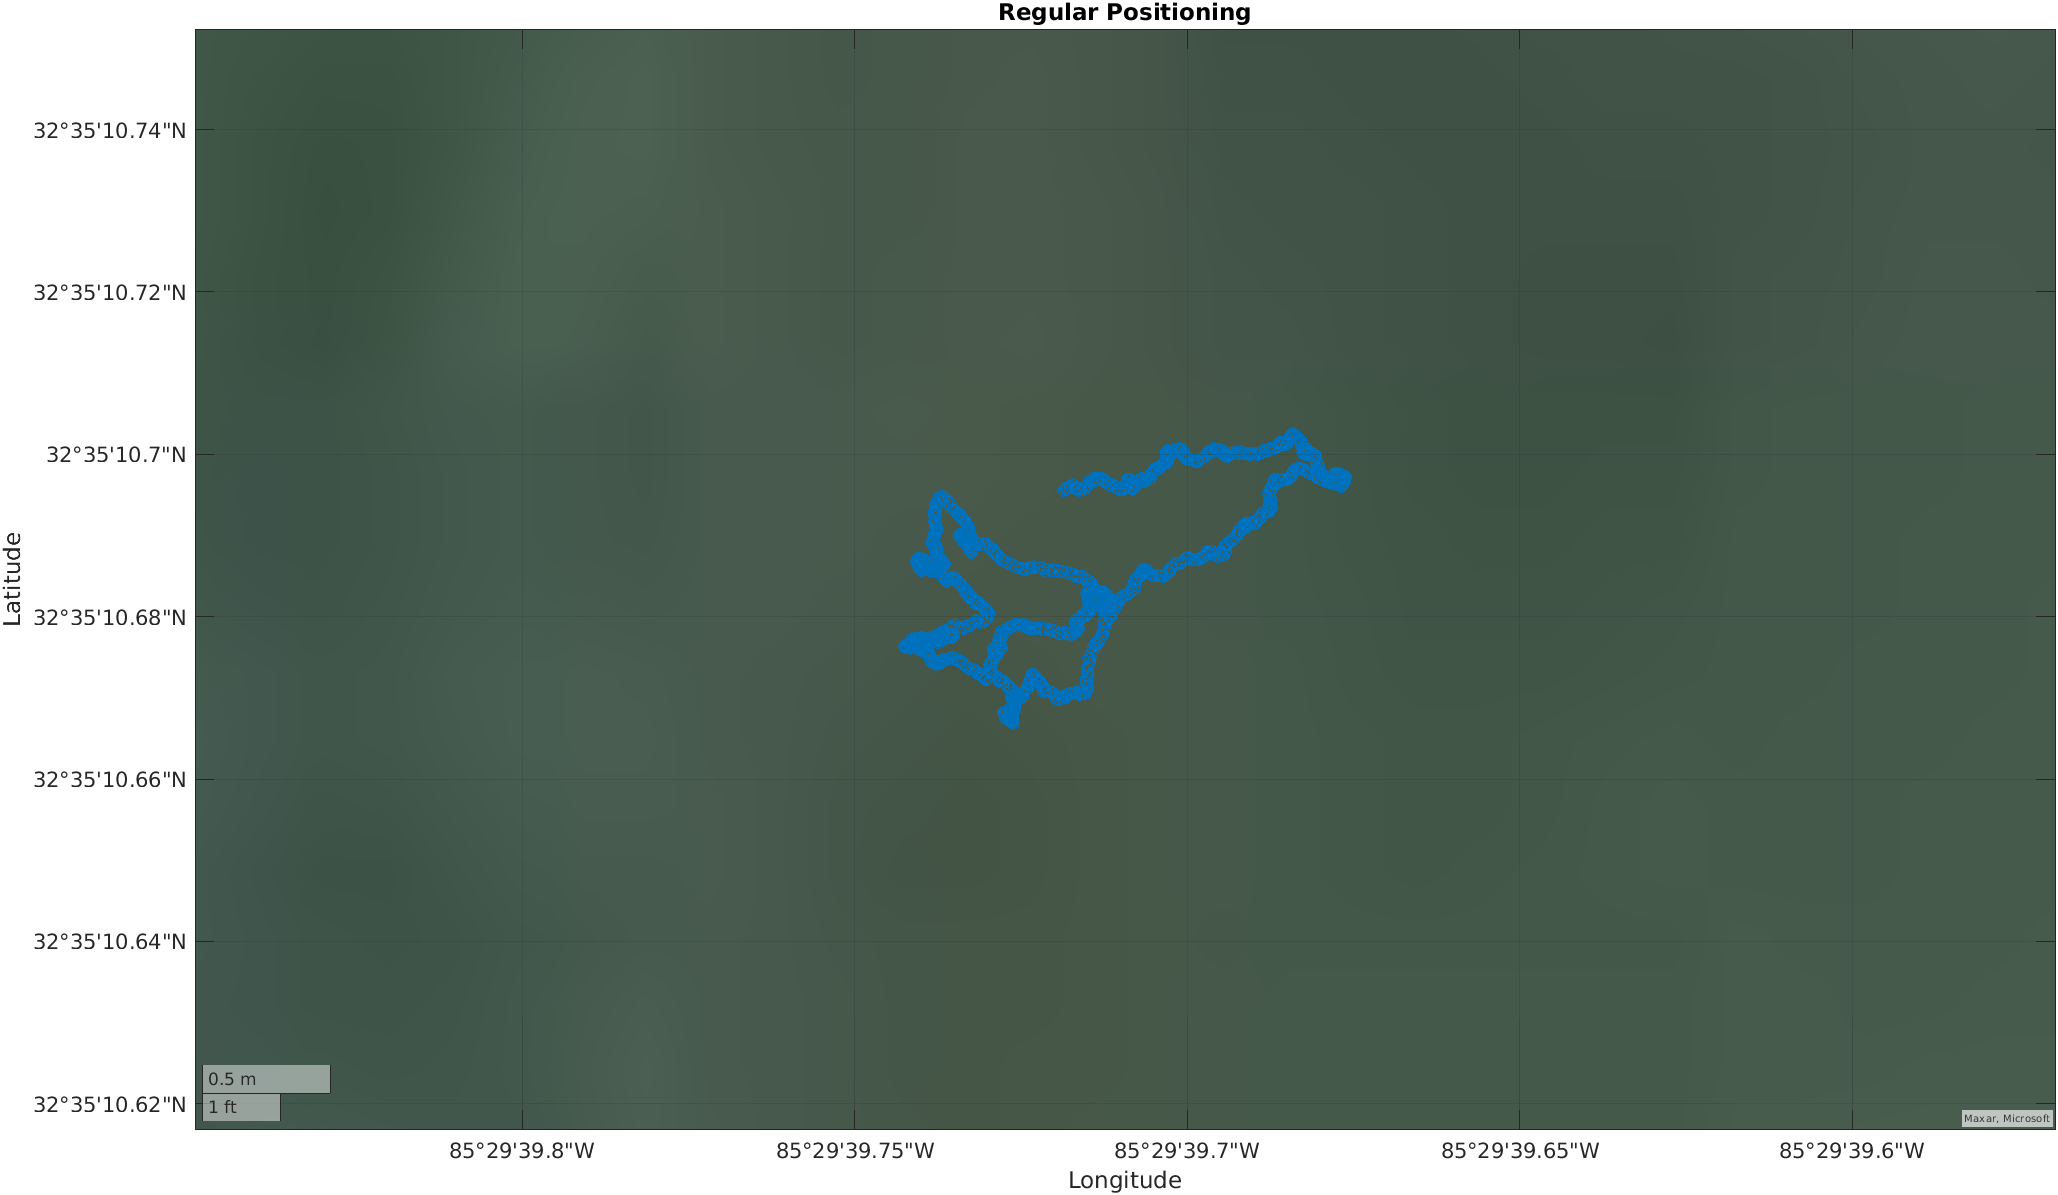
\includegraphics[width=0.85\textwidth]{p1_a.png}
        \caption{Static GPS Position Solution.}
    \end{figure}
    After determining the static GPS position solution carrier phase smoothing 
    was performed to mitigate the measurement noise. Carrier phase smoothing 
    utilizes the relative distance on a less noisy carrier phase measurement 
    to average the pseudorange over a window. The equation for carrier phase 
    smoothing is given as:
    \begin{equation}
      \bar{\rho}(t_i ) = \dfrac{1}{M} \rho(t_i)+\dfrac{M-1}{M}
      \left[\bar{\rho}(t_i-1) + \phi(t_i) - \phi(t_i-1)\right]
    \end{equation}
    where $\bar{\rho}$ is the averaged pseudorange, $M$ is the averaging window, 
    $t_i$ is the current time step, and $\phi$ is the carrier phase. Increasing 
    the averaging window allows for more smoothing but could introduce a bias. 
    Therefore window sizes of 2, 8, and 15 minutes were used as averaging windows 
    and compared against each other. To generate a position solution the same 
    Gauss-Newton least squares method is used but with the averaged pseudorange. 
    \emph{Figure 2} shows the carrier phase smoothed GPS position solutions for 
    each averaging window along with the regular GPS position solution. 
    \begin{figure}[H]
      \centering
      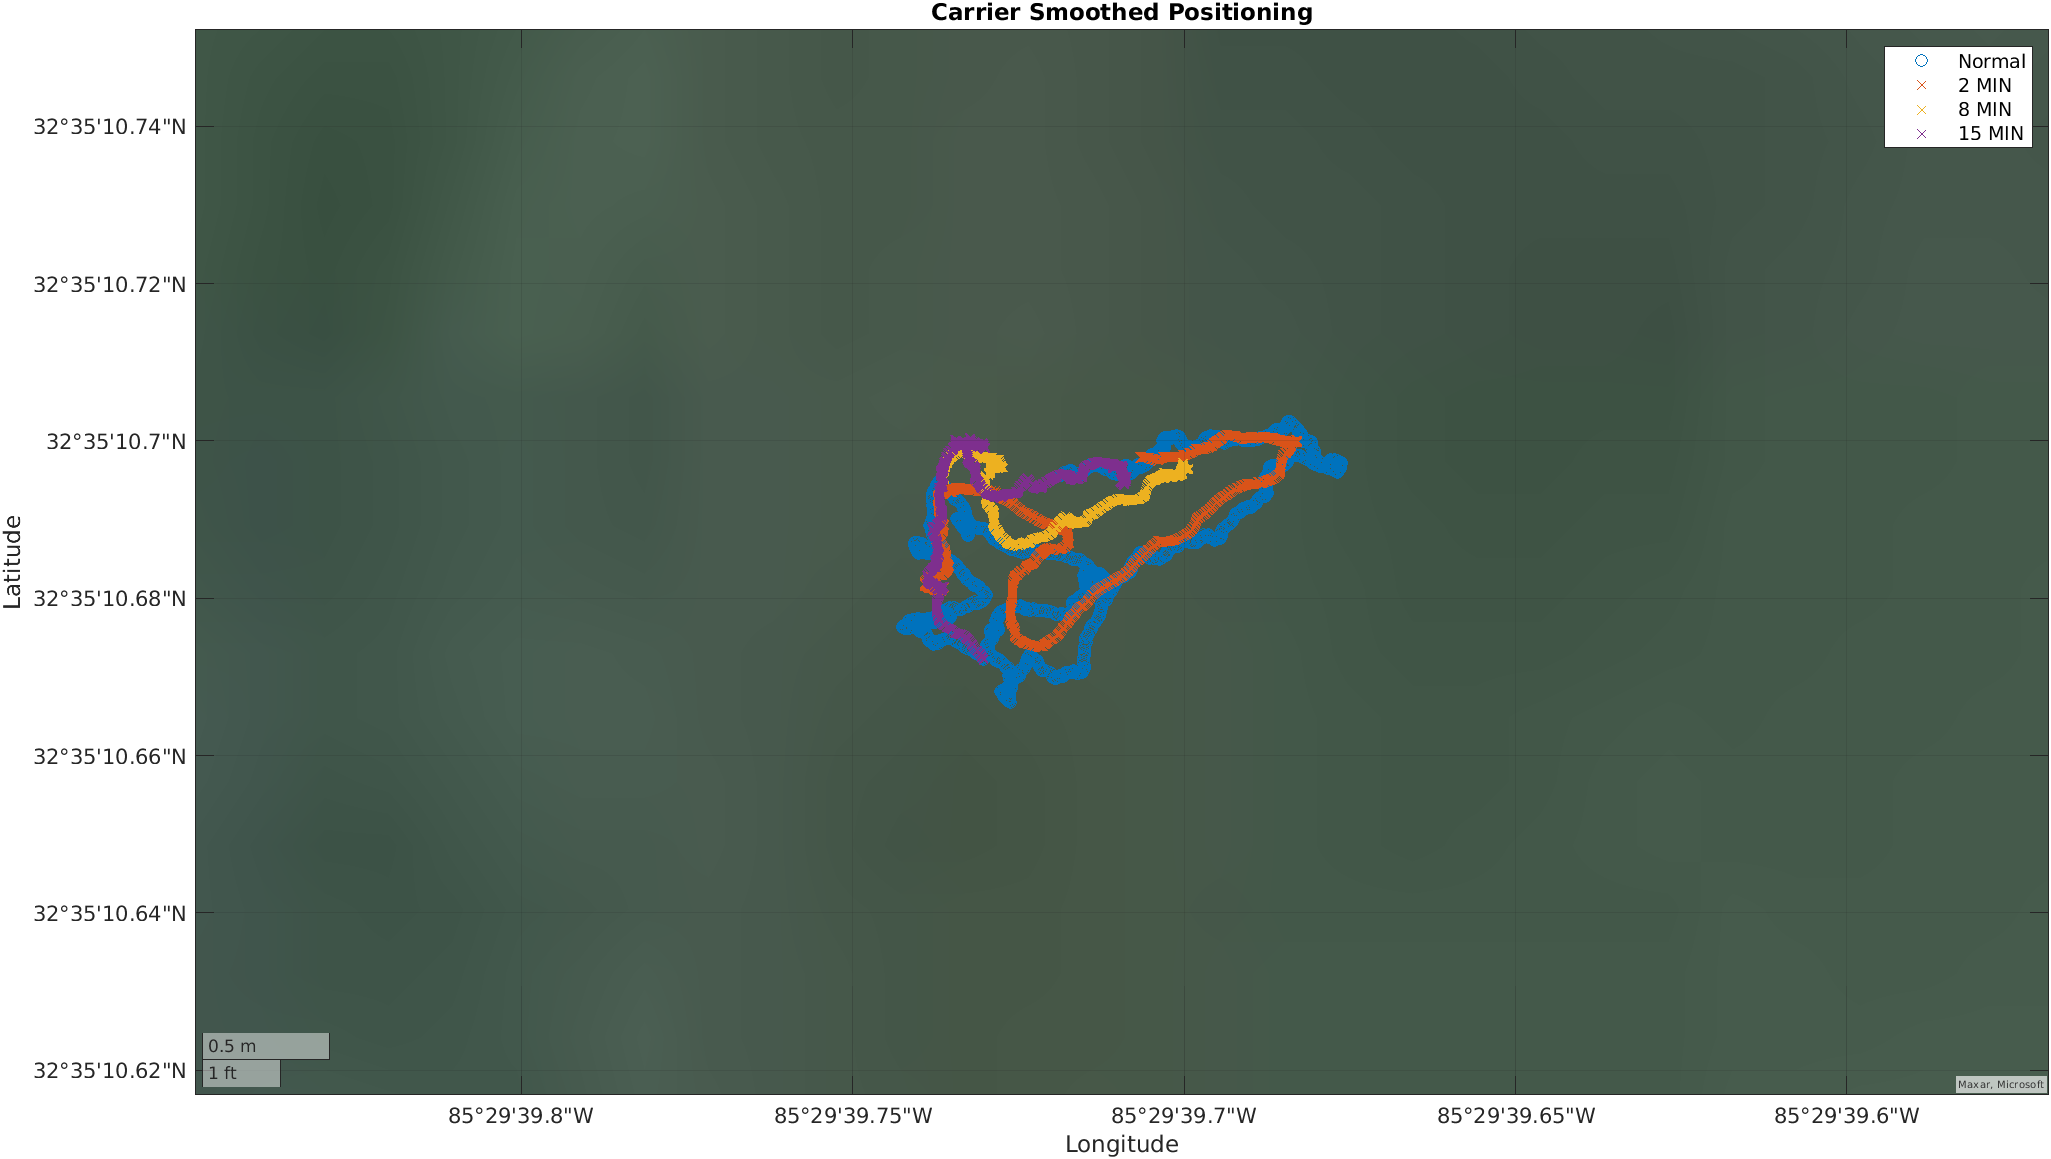
\includegraphics[width=0.85\textwidth]{p1_b.png}
      \caption{Carrier Smoothing GPS Position Solution.}
    \end{figure}
    From \emph{Figure 2}, it can be seen that increasing the averaging window 
    tightens the position solution. A smoother pseudorange measurement limits the 
    amount of variance on the position solution. For the static scenario, an 
    inclusion of a new bias is not seen for any of the averaging windows. 
    Therefore, the higher 15 minute averaging window would be the preferred 
    averaging window.
    \\ \\
    The next method used to reduce the static position error was implementing an 
    ephemeris ionosphere error model. This method estimates the atmospheric error 
    due to the ionosphere and removes it from the pseudorange measurements. The 
    equation for calculating the ionosphere correction term, taken from the GPS 
    Interface Control Document 
    (\url{https://eng.auburn.edu/~dmbevly/fund_gps/IonosphereCorrectionAlgorithm.pdf}) 
    is given as:
    \begin{equation}
      T_{iono}=
      \begin{cases}
        F*\left[5(10^{-9})+AMP(1-\dfrac{x^2}{2}+\dfrac{x^4}{24})\right], & |x|<1.57 \\
        F*\left[5(10^{-9})\right] & |x|\geq 1.57
      \end{cases}
    \end{equation}
    where $T_{iono}$ is the ionosphere correction term, $F$ is the obliquity 
    factor, and $x$ is the phase. This ionosphere is subtracted from the 
    pseudorange, and a new position solution is calculated. \emph{Figure 3} shows 
    the GPS position solution using the ephemeris ionosphere model correction as 
    well as the original GPS position solution.
    \begin{figure}[H]
      \centering
      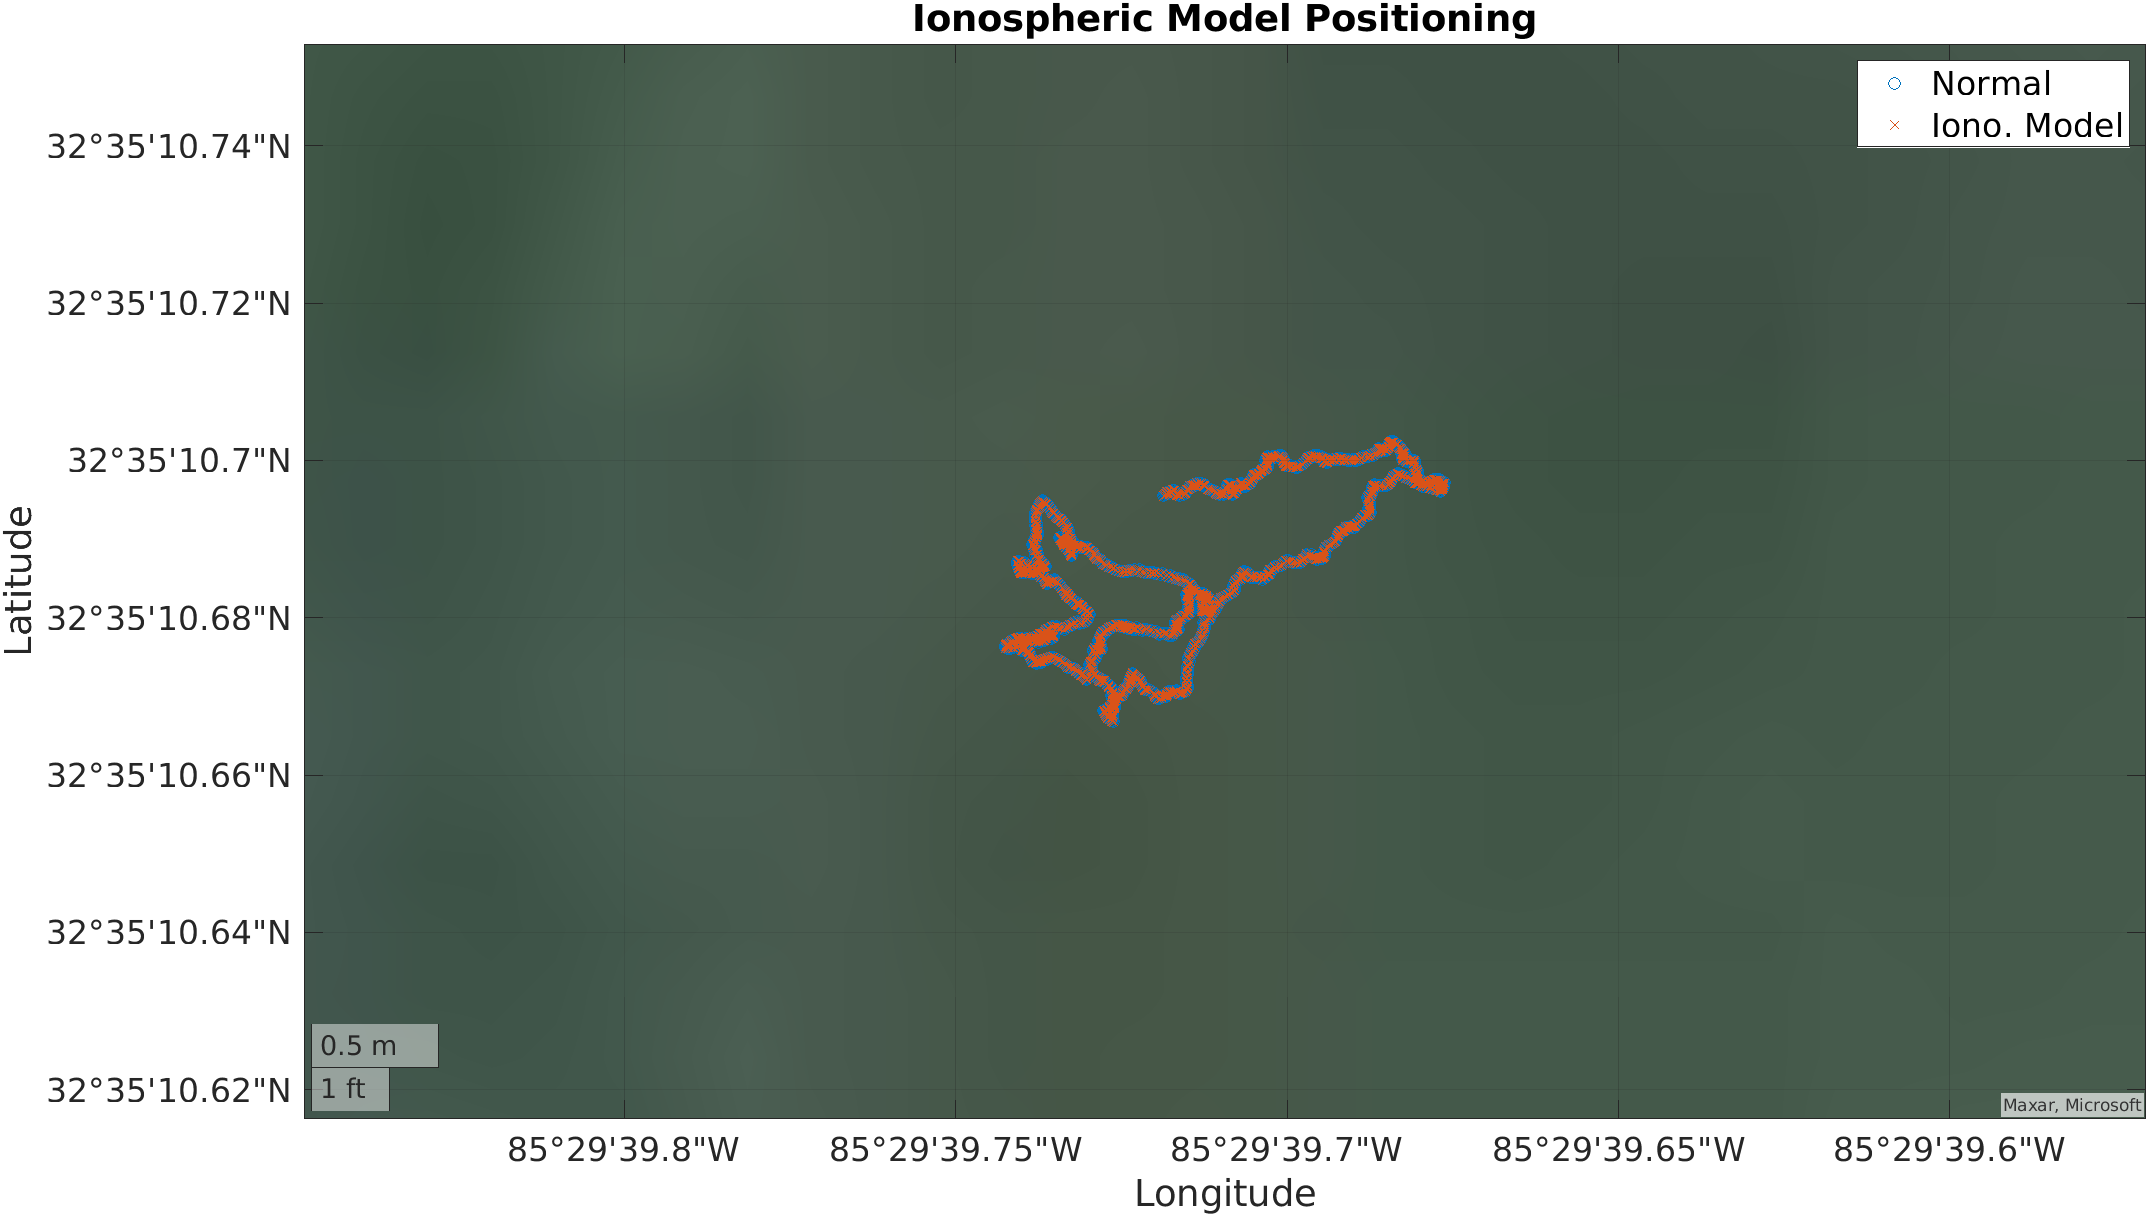
\includegraphics[width=0.85\textwidth]{p1_c.png}
      \caption{Ephemeris Model Correction GPS Position Solution.}
    \end{figure}
    The ephemeris ionosphere model correction did not have much of an effect 
    on the position solution. This is due to low amounts of ionosphere error 
    being present in the data set to begin with. Another method of mitigating 
    the ionosphere error is to use dual frequency to produce ionosphere free 
    measurements. The error due to the ionosphere differs based on the signal 
    frequency. By comparing pseudorange measurements at different frequencies, 
    the error due to the ionosphere can be ascertained. The equation for an 
    ionosphere free pseudorange is given by:
    \begin{equation}
      \rho_{IF} = \dfrac{f_{L1}^2}{(f_{L1}^2-f_{L2}^2)}\rho_{L1} - 
                  \dfrac{f_{L2}^2}{(f_{L1}^2-f_{L2}^2)}\rho_{L2}
    \end{equation}
    where $\rho_{IF}$ is the ionosphere free pseudorange, $f_{L1}$ is the L1 
    frequency, and $f_{L2}$ is the L2 frequency. This ionospehere free pseudorange 
    is used to create a new position solution. \emph{Figure 4} shows the GPS 
    position solution using the dual frequency ionosphere free measurements and 
    the original position solution. 
    \begin{figure}[H]
        \centering
        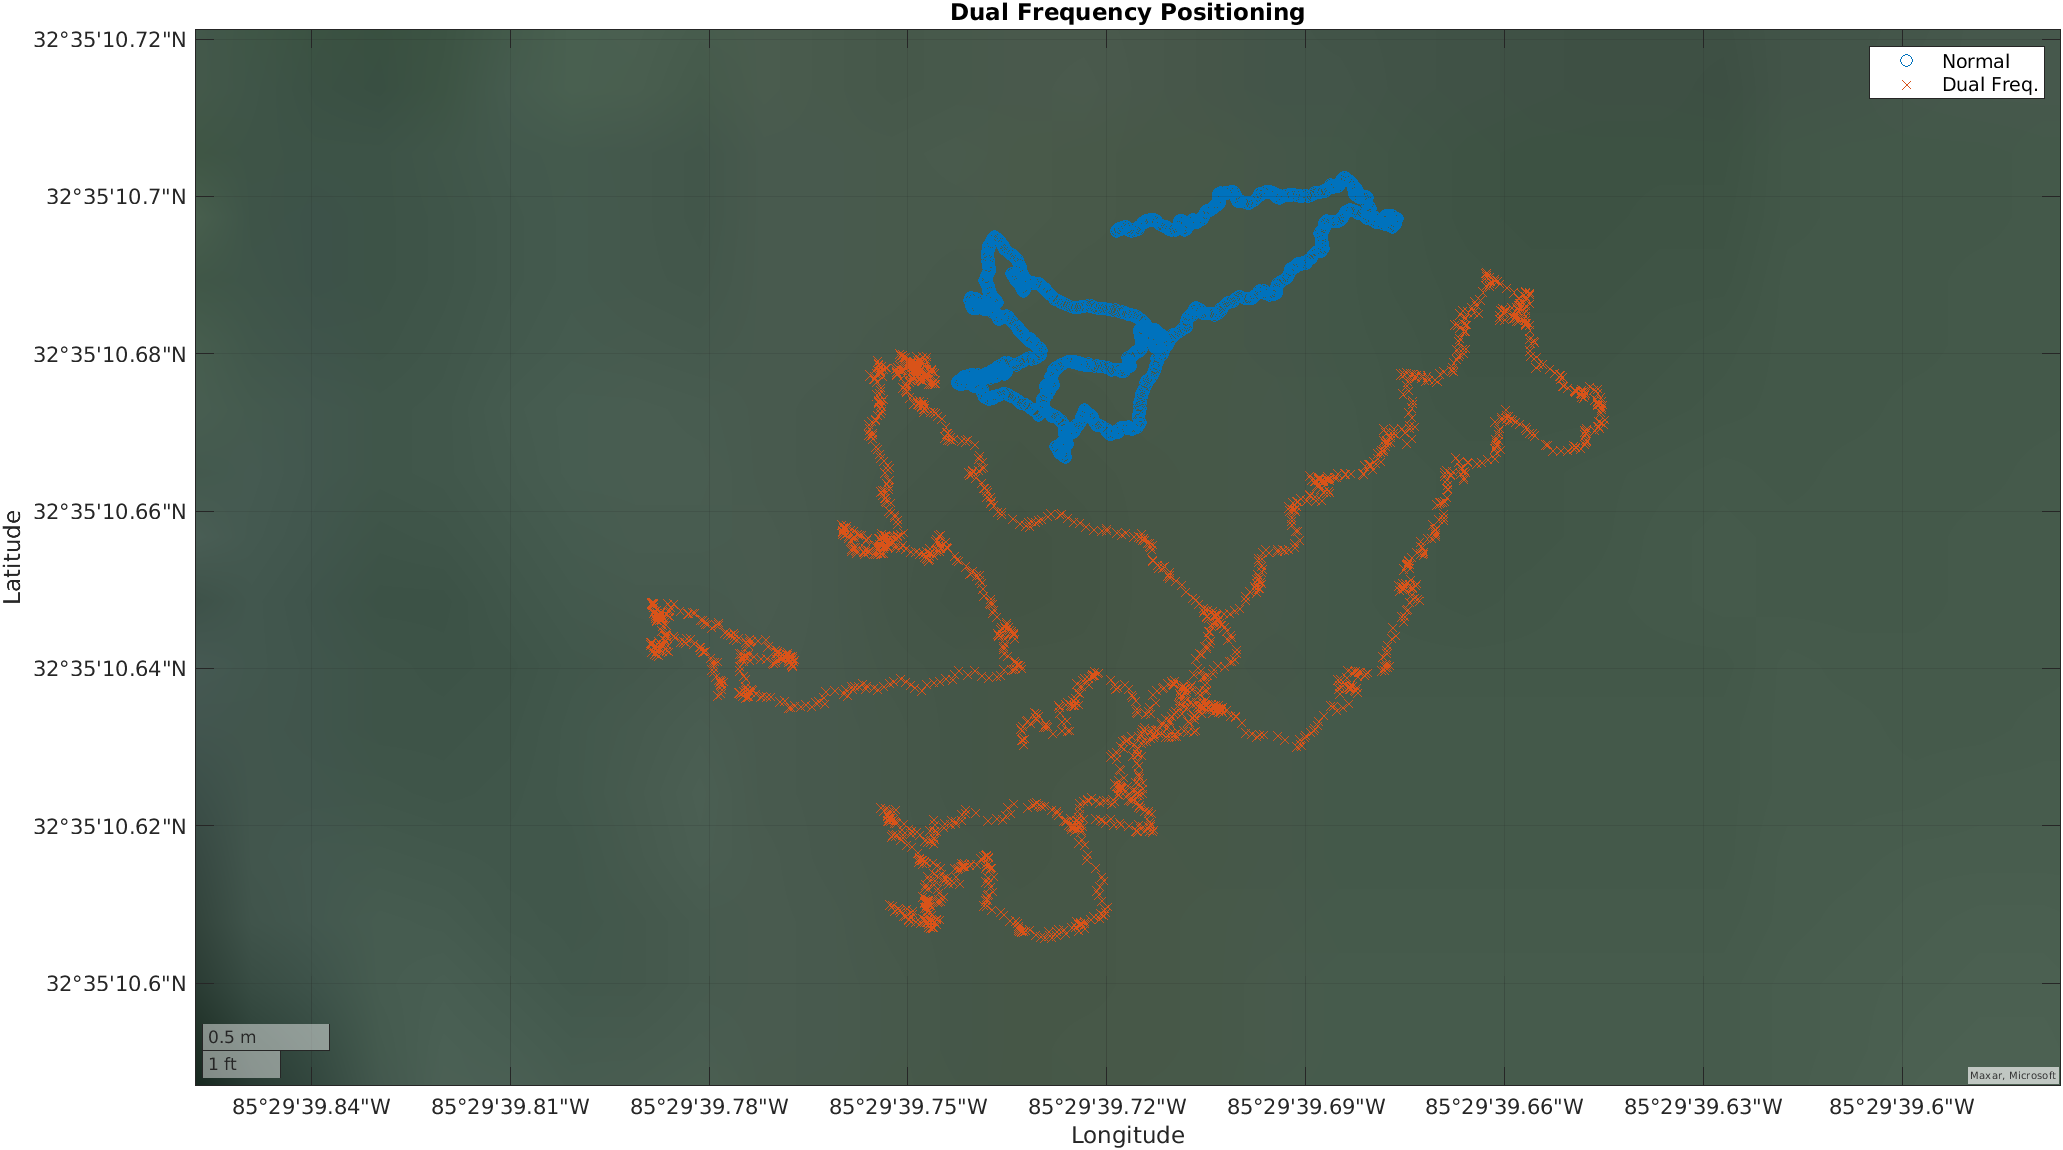
\includegraphics[width=0.85\textwidth]{p1_d.png}
        \caption{Dual Frequency Ionosphere Free GPS Position Solution.}
    \end{figure}
    From \emph{Figure 4} it can be seen that the position solution with the 
    ionosphere free measurements moves to a new general location. This is due to 
    the removal of the ionosphere error. However, it is also shown that the new 
    position solution is scattered much more when compared to the original position 
    solution. Since the error is added from both the L1 and L2 signals, the 
    position solution will show more variance. 
    \\ \\
    Each of the static positions solutions are plotted against each other in 
    \emph{Figure 5}. Additionally, \emph{Table 1} gives the mean position in latitude 
    and longitude as well as the standard deviation of the ECEF positions.
    \begin{figure}[H]
        \centering
        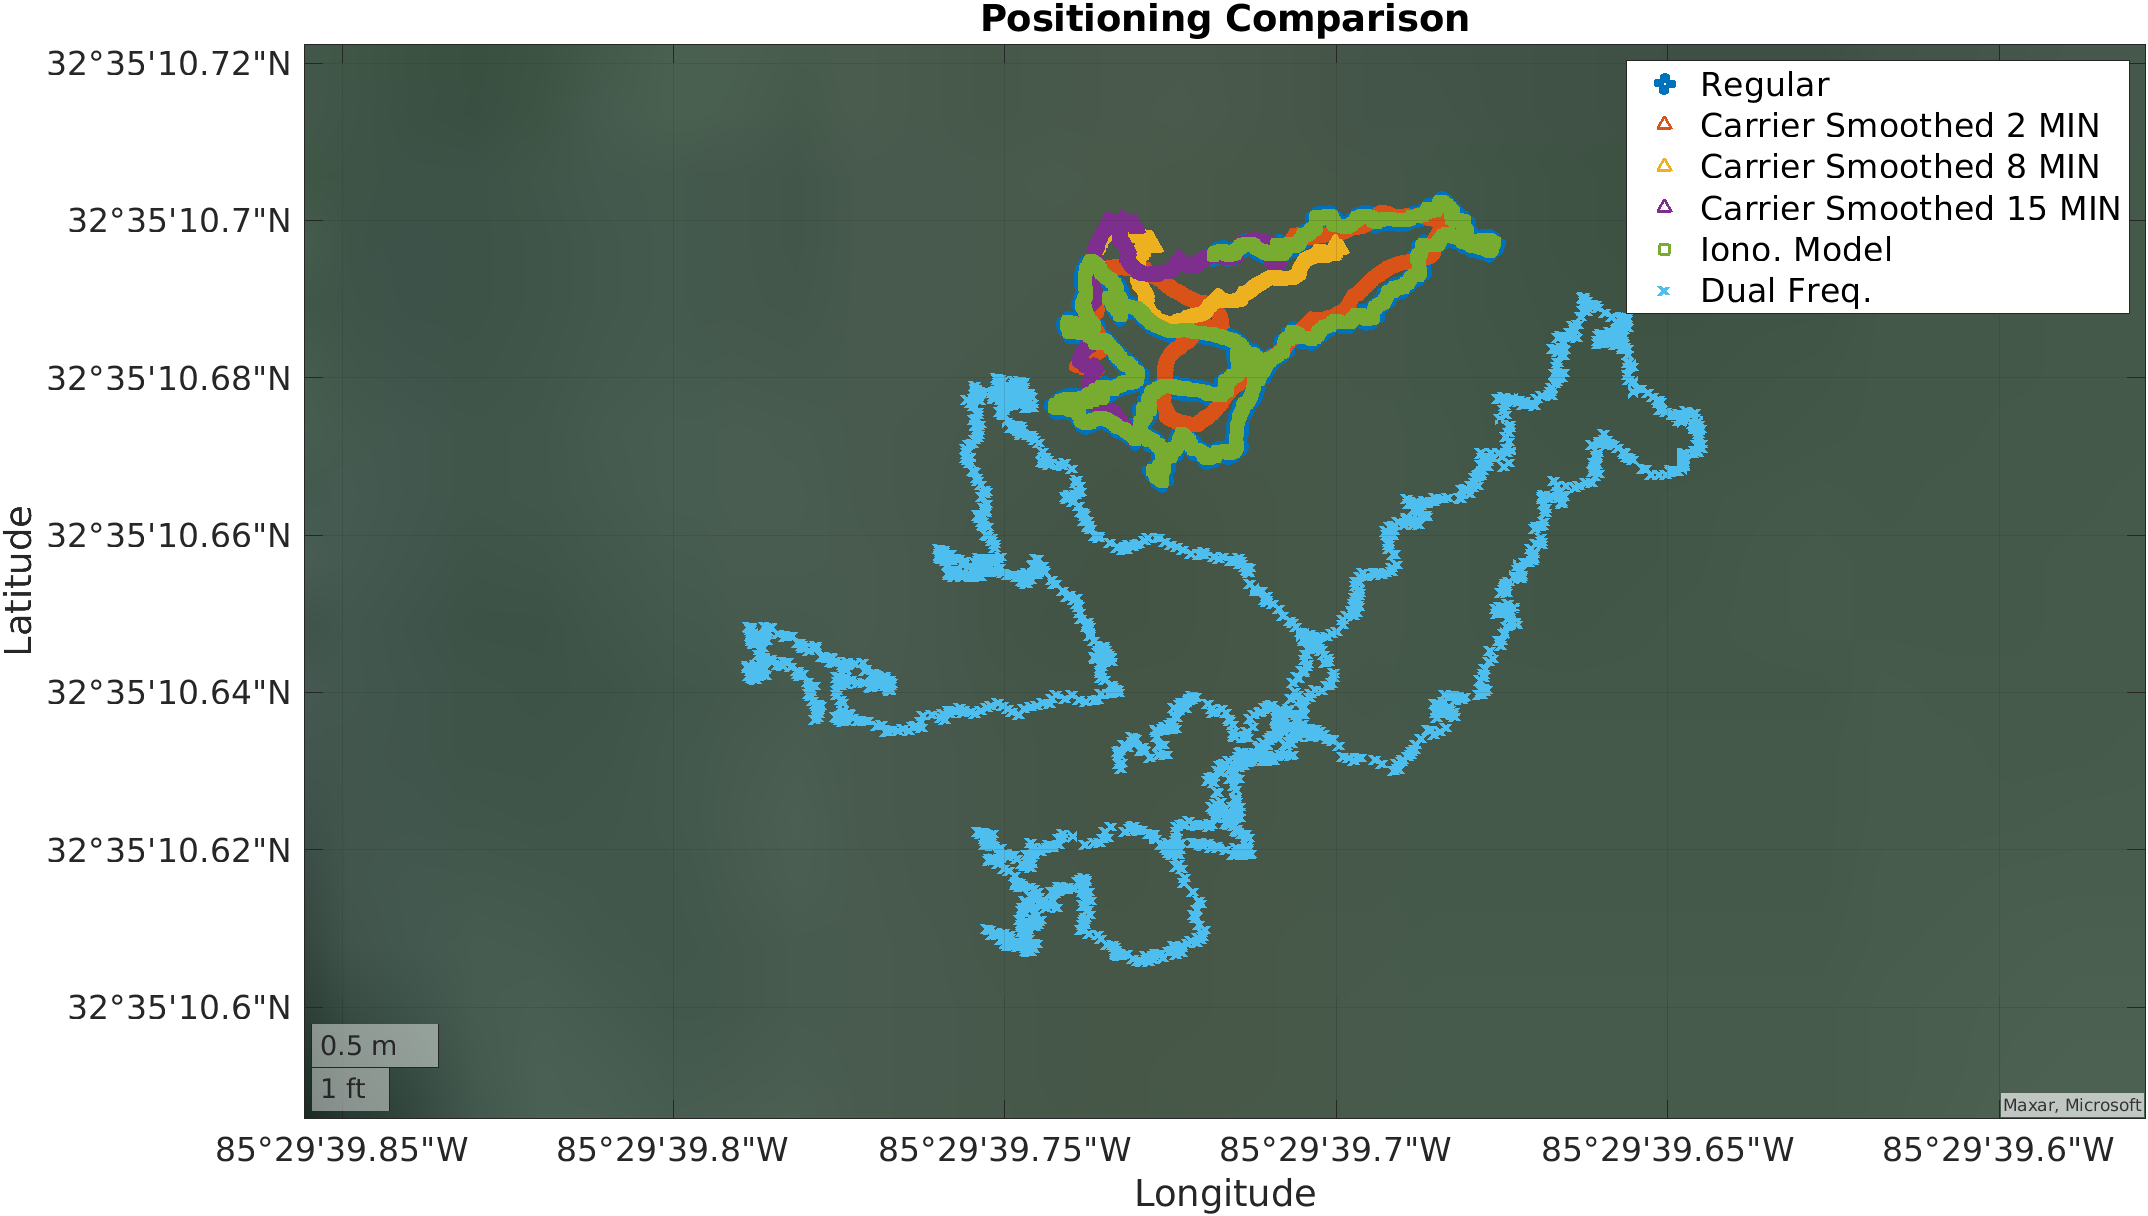
\includegraphics[width=0.85\textwidth]{p1_f.png}
        \caption{Dual Frequency Ionosphere Free GPS Position Solution.}
    \end{figure}
    % \rowcolors{2}{white}{lightgray}
    \begin{table}[H]
      \centering
      \caption{Statistics for Static Position Solutions.}
      \begin{tabular}{ P{4.25cm}|P{2.5cm} P{2.5cm} P{1.5cm} P{1.75cm} P{1.5cm} }
          & \boldmath$\mu_{\phi}$ (\degree) & \boldmath$\mu_{\lambda}$ (\degree) & \boldmath$\sigma_{x}$ (m) & \boldmath$\sigma_{y}$ (m) & \boldmath$\sigma_{z}$ (m) \\
        \hline
        \textbf{Regular} & \multicolumn{5}{c}{} \\
        L1 Position & 32.586302 & -85.494366 & 0.533 & 0.651  & 0.734 \\
        \hline
        \textbf{Carrier Smoothing} & \multicolumn{5}{c}{} \\
        2 min & 32.586302 & -85.494366    & 0.509  & 0.553   & 0.624  \\
        8 min & 32.586303 & -85.494368  & 0.362 & 0.191  & 0.318 \\
        15 min & 32.586304 & -85.494369  & 0.245 & 0.253 & 0.245 \\
        \hline
        \textbf{Ionosphere Correction} & \multicolumn{5}{c}{} \\
        Ephemeris Model & 32.586302 & -85.494366 & 0.533 & 0.652  & 0.734  \\
        Dual Frequency & 32.586291 & -85.494367  & 0.946 & 1.391 & 1.252 \\
      \end{tabular}
    \end{table}
    % \\ \\ \\
    From \emph{Figure 5} and \emph{Table 1} it can be seen that each of the 
    position solutions are located in a similar location. The only position 
    solution that is located farther than 1 meter away from the others is the 
    dual frequency position solution. The dual frequency positioning is on 
    average about 8 meters away from the original positioning solution. This 
    is due to the removal of the ionosphere error, which removes a bias in the 
    measurements. However, this position solution also has the highest standard 
    deviation. This is due to the noise on the measurements being increased 
    since two different pseudoranges are used. The positioning solution with 
    the lowest standard deviation is the carrier smoothed positioning solution 
    with a 15 minute averaging window. The noise on the measurements was 
    mitigated using the more precise carrier phase measurements, leading to 
    less position variance. The ionosphere model position solution has the 
    least amount of impact on the original solution. The mean and standard 
    deviation for each position solution are about the same. This is because 
    the calculated ionosphere correction term for was small for the entire 
    data set. To remove both the noise and bias on the original position 
    solution, using a mix of the dual frequency and carrier smoothing methods 
    would be the most ideal.

  \item \textbf{Static Relative DGPS Positioning} \\
    Differential GPS (DGPS) techniques can utilize the same techniques used in single 
    receiver positioning. To begin, a single receiver positioning solution was 
    done using \emph{Equation 1} as a baseline for all DGPS techniques. This is 
    presented in \emph{Figure 6}. Note that for this entire section, two receivers 
    were connected to the same antenna, therefore the distance between the receivers 
    should be 0 meters.
    \begin{figure}[H]
      \centering
      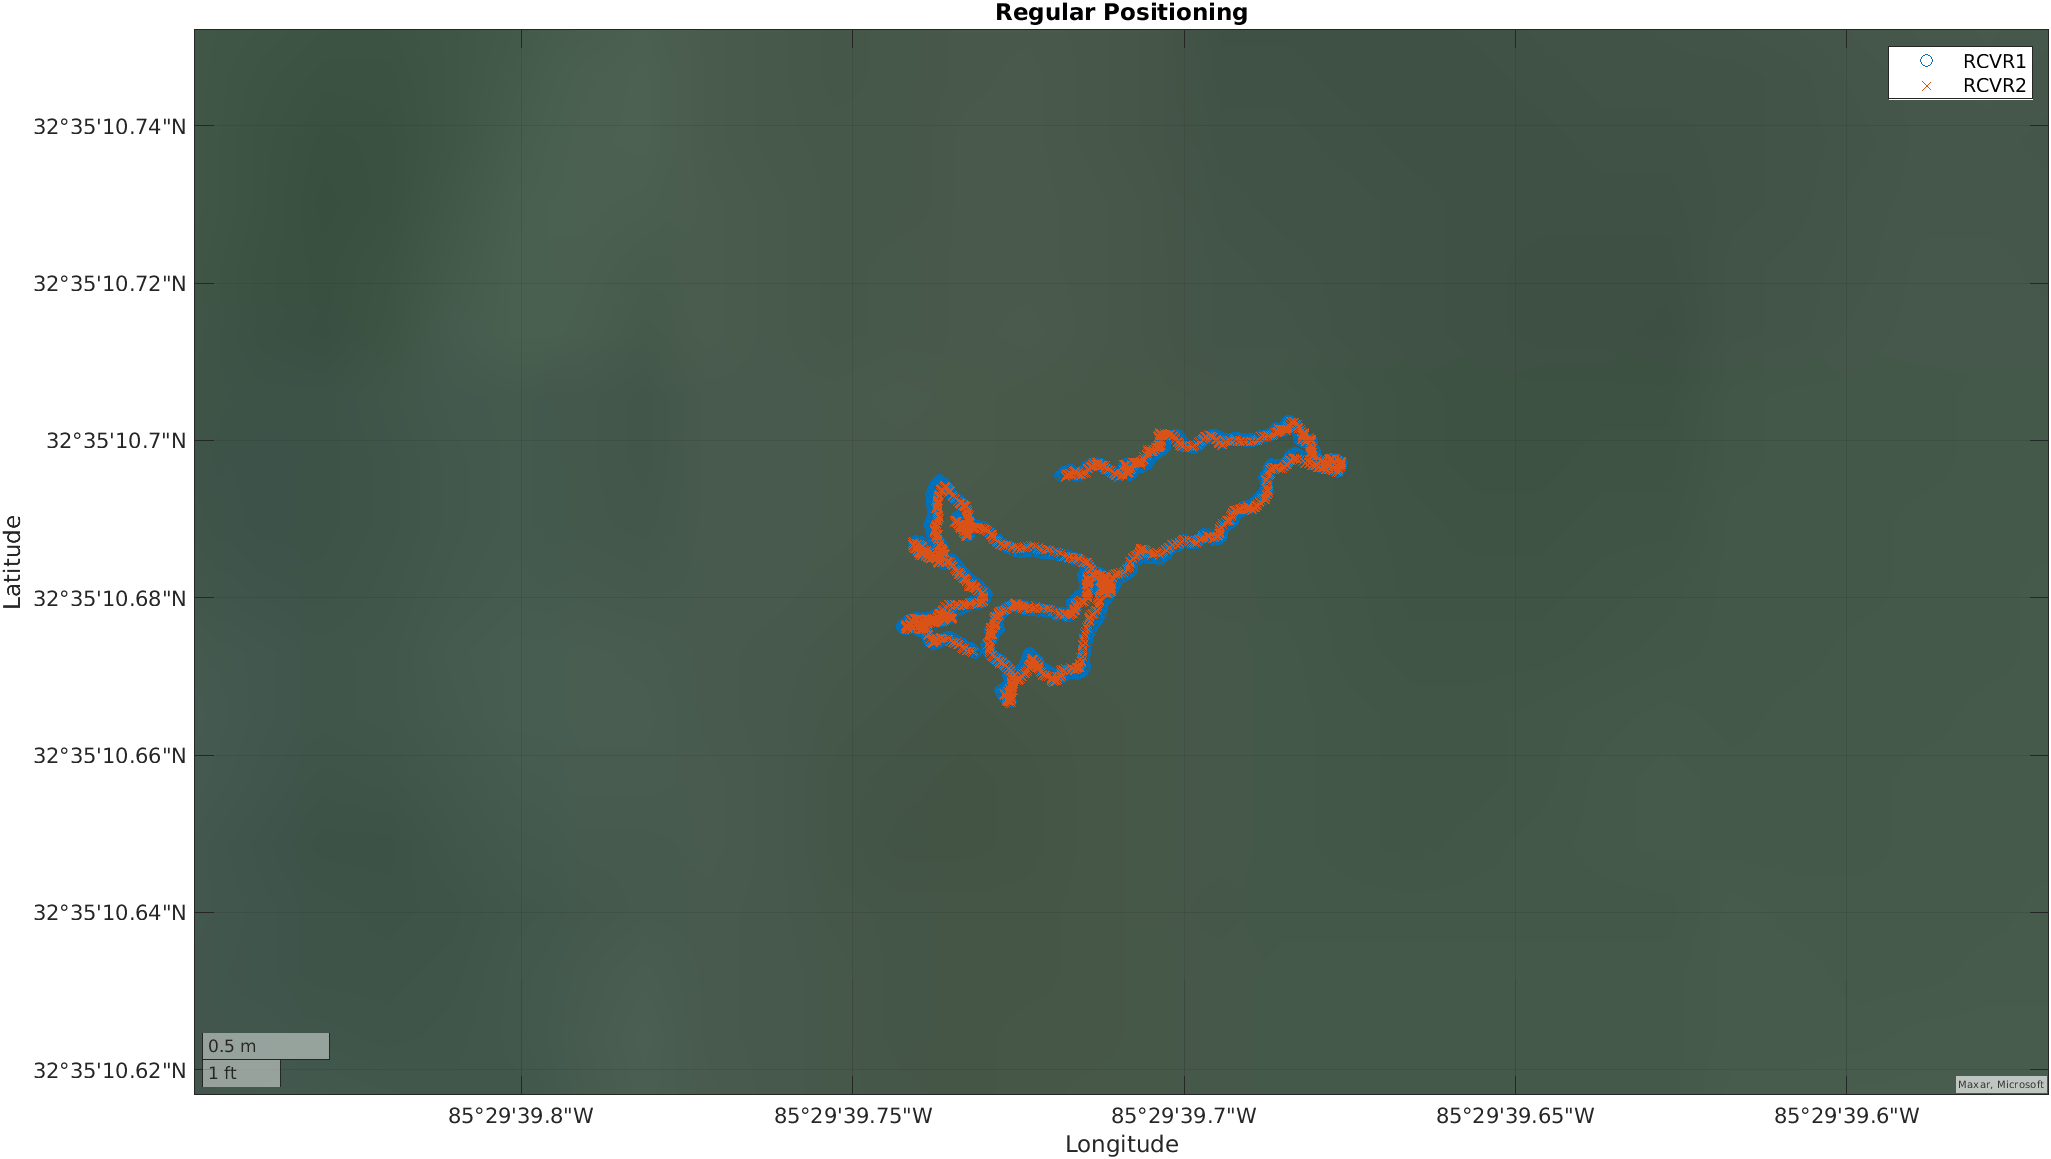
\includegraphics[width=0.85\textwidth]{p2_a.png}
      \caption{Static Position of Two Receivers.}
    \end{figure}
    Next, the DGPS solution was created using RCVR\_S2 as the base station. This was 
    determined via the linear least squares solution below.
    \begin{equation}
      \delta\rho = 
      \begin{bmatrix}
        u_x & u_y & u_z & 1
      \end{bmatrix}
      \begin{bmatrix}
        r_x \\ r_y \\ r_z \\ c \delta t \\
      \end{bmatrix}
    \end{equation}
    Where $\delta\rho$ is the psuedorange difference between the receivers, $u$ are 
    the unit vectors of one receiver to the satellites, $r$ are the relative position 
    vectors from the first receiver to the second, and $c \delta t$ is the clock bias 
    difference between the receivers. \emph{Figure 7} shows the DGPS solution when using 
    RCVR\_S2 as the base station.
    \begin{figure}[H]
      \centering
      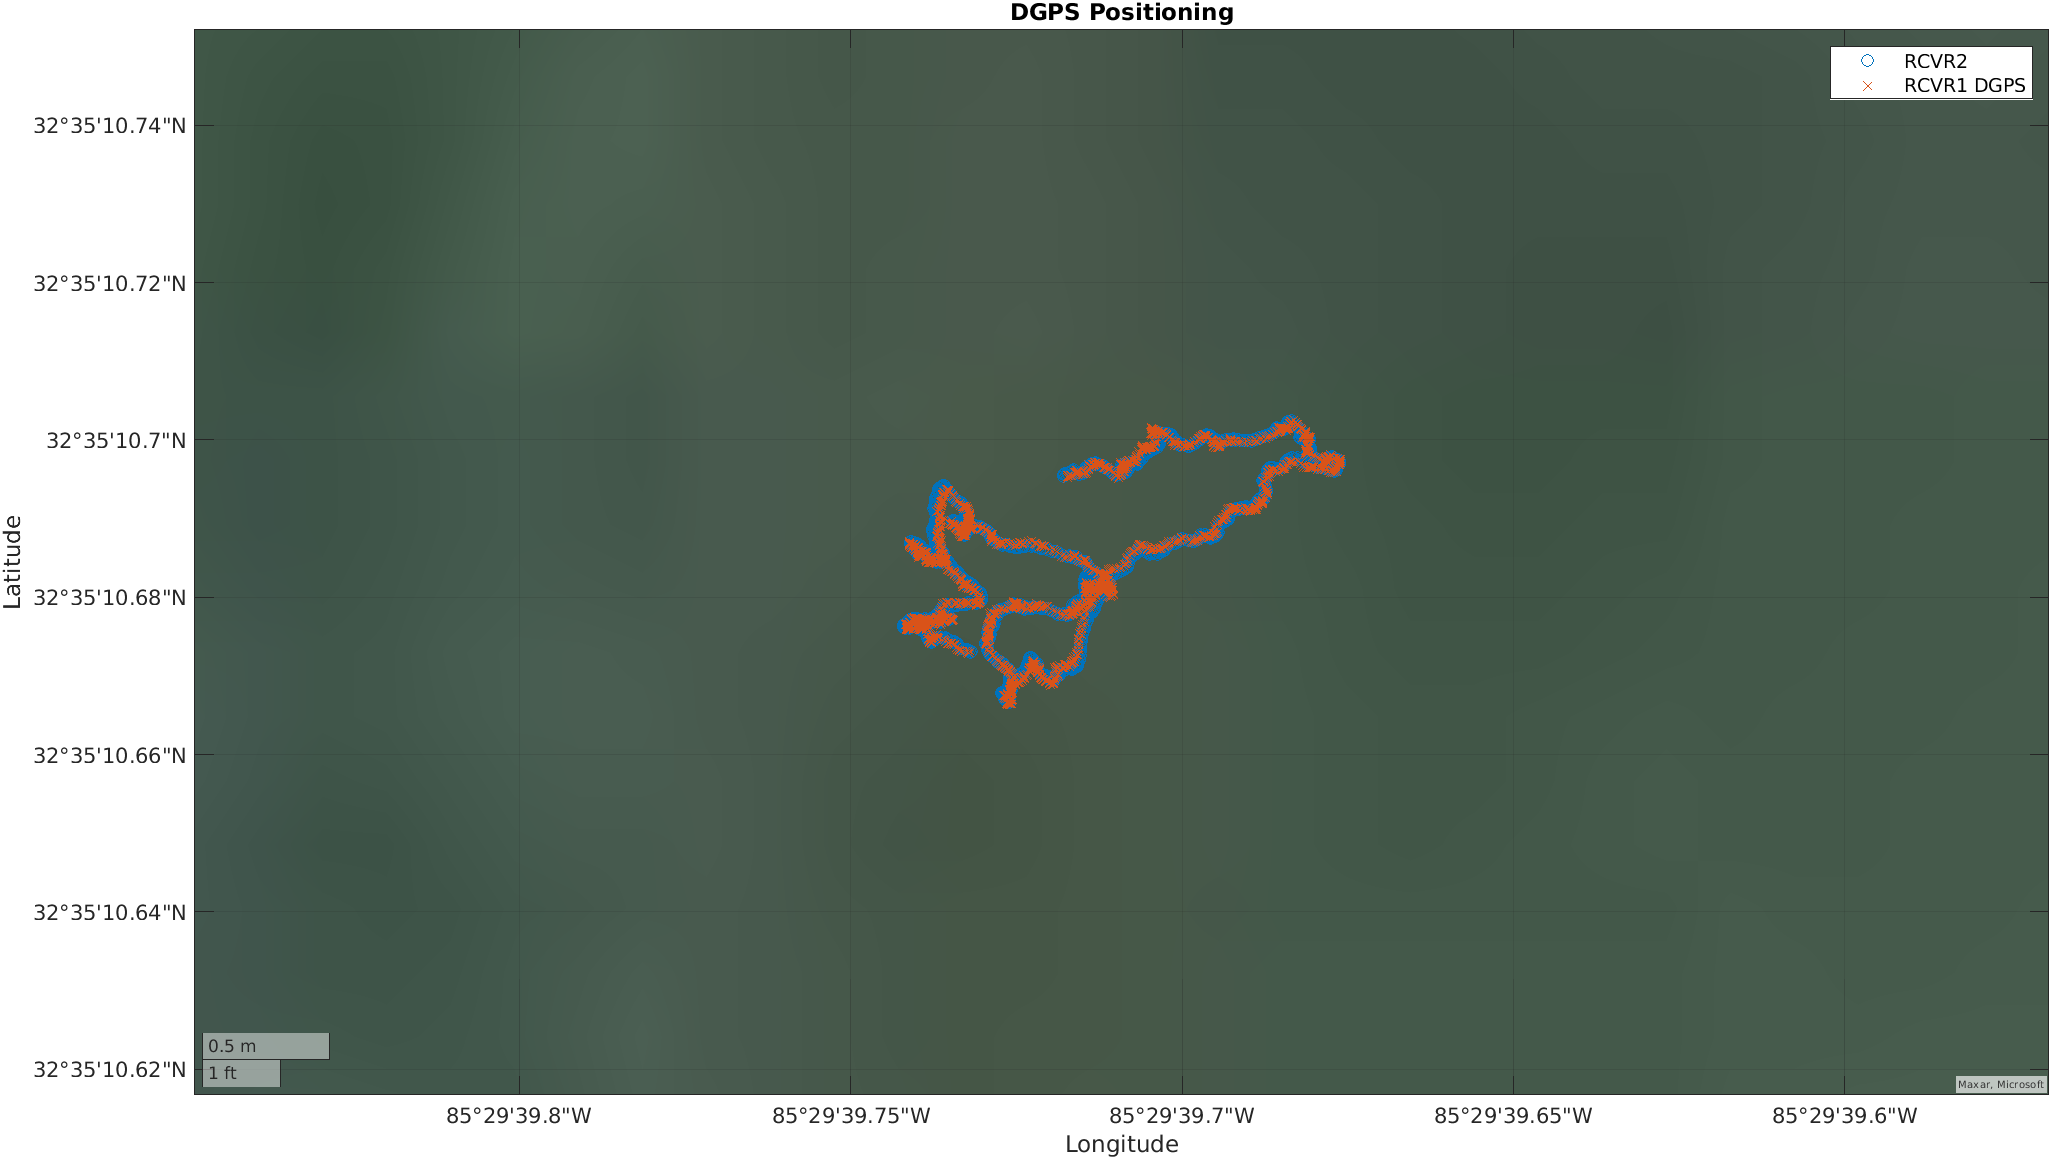
\includegraphics[width=0.85\textwidth]{p2_b.png}
      \caption{Static DGPS Solution.}
    \end{figure}
    As shown, the DGPS solution is almost identical to the reference solution as the 
    baseline between them is 0 meters and both receivers are connected to the same 
    antenna.
    \\ \\
    Carrier phase smoothing was again utilized to mitigate the measurement 
    noise on the pseudorange measurements. This time, however, the psuedorange and 
    carrier differences between the measurements were used as shown in 
    \emph{equation 6}.
    \begin{equation}
      \delta\bar{\rho}(t_i) = \dfrac{1}{M} \delta\rho(t_i) + 
                              \dfrac{M-1}{M} \left[\delta\bar{\rho}(t_{i-1}) + 
                              \delta\phi(t_i) - \delta\phi(t_{i-1})\right]
    \end{equation}
    Sizing widows of 2, 8, and 15 minutes were used and presented in \emph{Figure 8}. 
    The smoothing attempt on the DGPS solution has no visual impact on the 
    positioning solution, likely due to the small differences in the measured 
    psuedoranges  and carrier from the receivers which leads to the smoothing having 
    minimal effect on the solution.
    \begin{figure}[H]
      \centering
      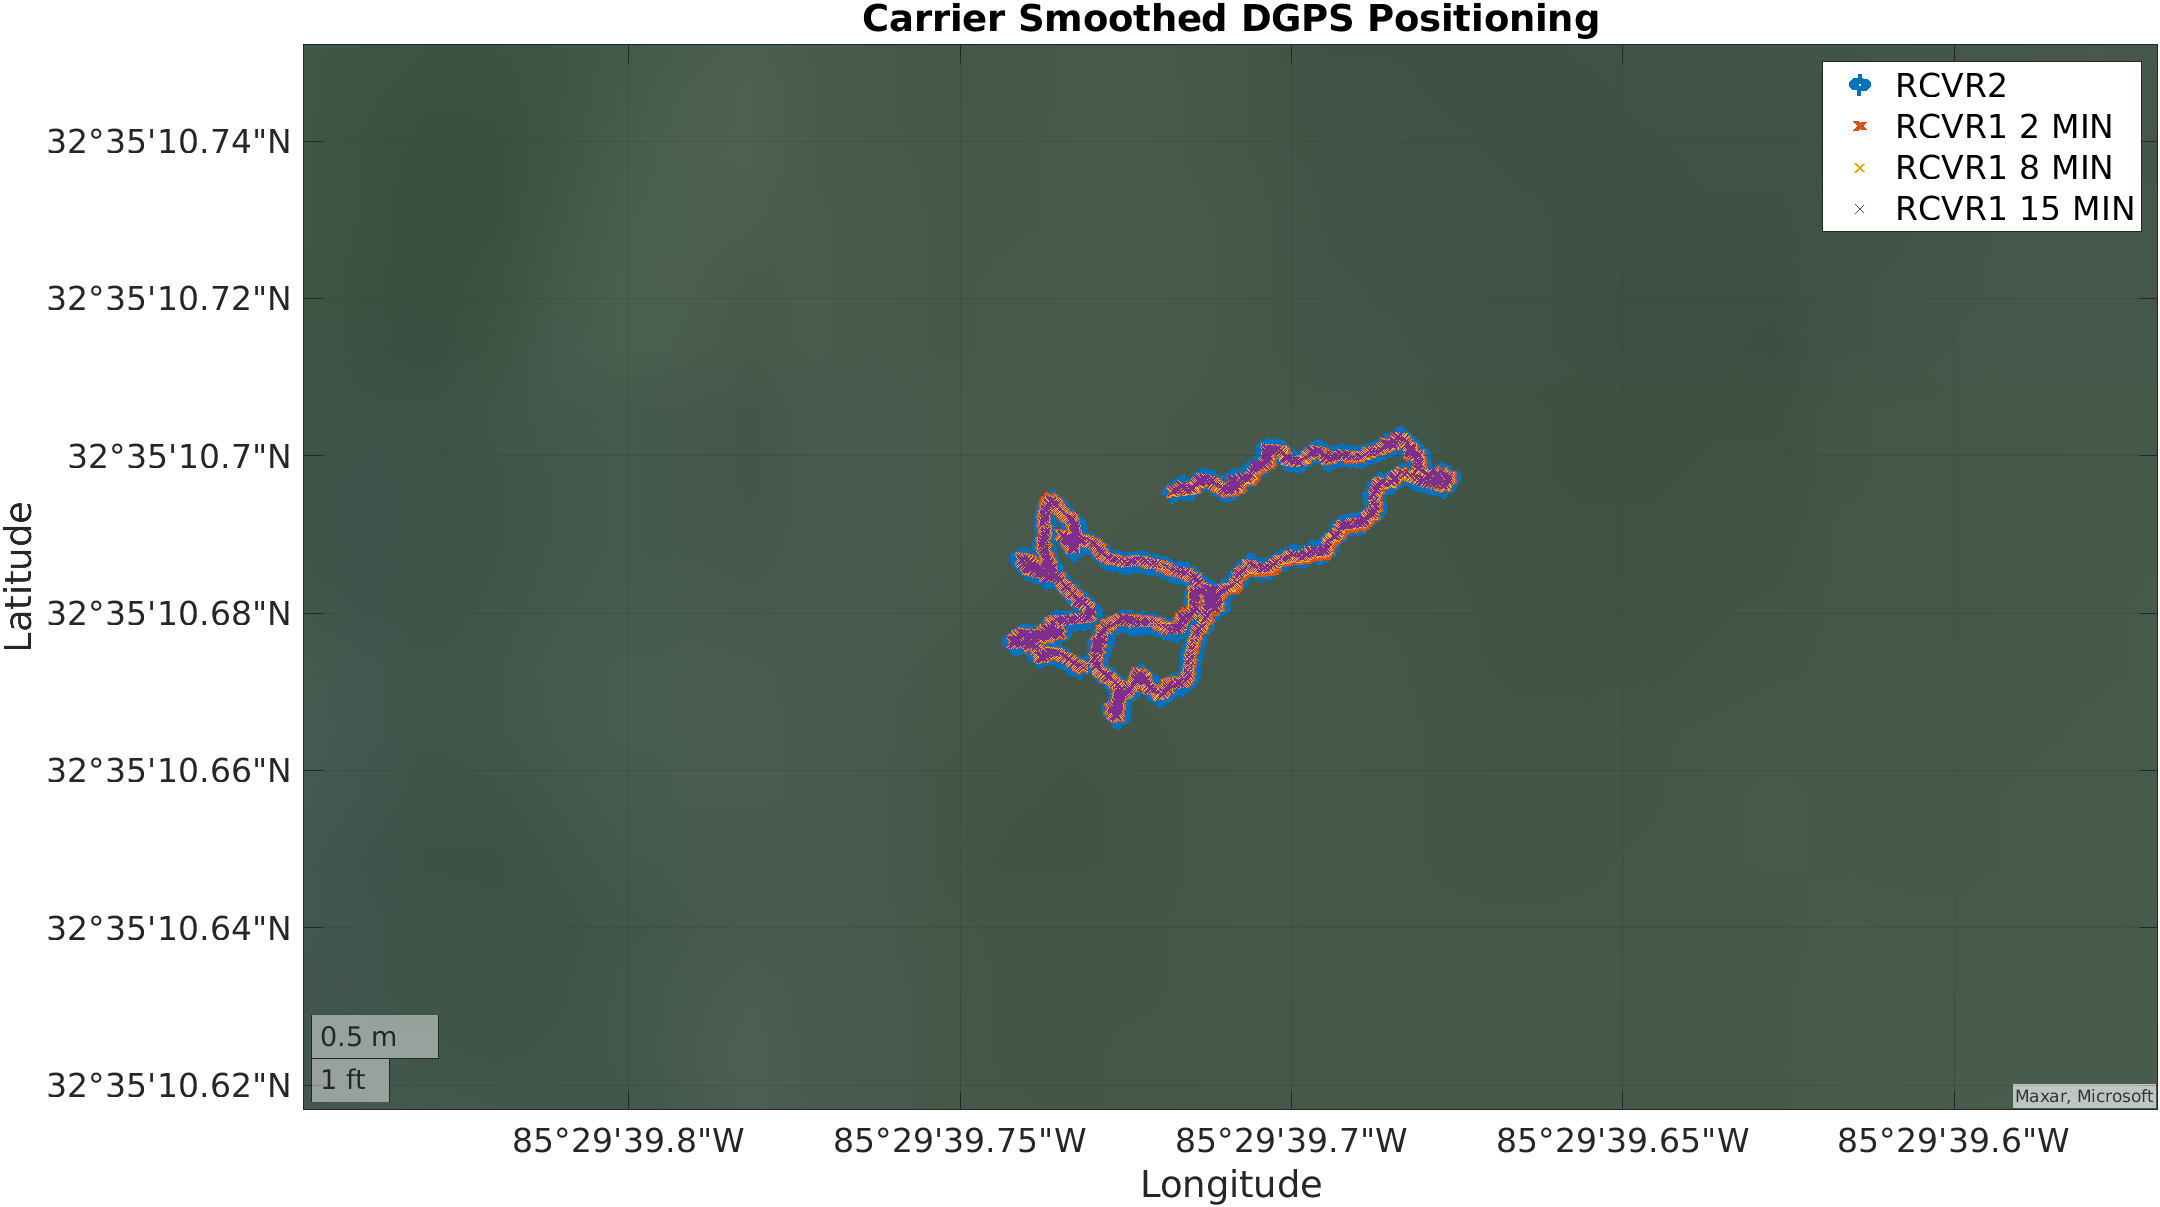
\includegraphics[width=0.85\textwidth]{p2_c.png}
      \caption{Static Carrier Smoothed DGPS Solution.}
    \end{figure}
    Lastly, a RTK DGPS solution was used to position the two receivers. This utilized 
    carrier measurements by attempting to first estimate the integer ambiguity seen in 
    the measurement as shown.
    \begin{equation}
      \delta \phi = 
      \begin{bmatrix}
        u_x & u_y & u_z & 1
      \end{bmatrix}
      \begin{bmatrix}
        r_x \\ r_y \\ r_z \\ c \delta t \\
      \end{bmatrix}
      + \lambda \delta N
      = G \delta r + \lambda \delta N
    \end{equation}
    Where $\lambda$ is the carrier wavelength and $\delta N$ is the estimated integer 
    ambiguity between the receivers. Using the L1 psuedorange measurement along with 
    the L1 and L2 carrier measurements, the integer ambiguity can be solved for as 
    follows:
    \begin{equation}
      \begin{bmatrix}
        \delta \rho_{L1} \\ \delta \phi_{L1} \\ \delta \phi_{L2}
      \end{bmatrix}
      =
      G \delta r +
      \begin{bmatrix}
        0 & 0 \\ \lambda_{L1} & 0 \\ 0 & \lambda_{L2}
      \end{bmatrix}
      \begin{bmatrix}
        \delta N_{L1} \\ \delta N_{L2}
      \end{bmatrix}
    \end{equation}
    Separating the second half of the equation and solving for the integer ambiguity:
    \begin{equation}
      \begin{split}
        L &= leftnull(G) \\
        \delta N &= [(L\lambda)^T(L\lambda)]^{-1}(L\lambda)^T Ly \\
        P_{\delta N} &= [(L\lambda)^T(L\lambda)]^{-1}
      \end{split}
    \end{equation}
    This hand solution is a medium fidelity, potential solution, however, the Lambda method 
    was employed on this solution to provide an even more accurate solution. This solution 
    was implemented with the code provided by Delft University. \emph{Figure 9} is a plot 
    of the RTK DGPS solution from the Lambda method, which again shows little visual 
    improvement over the reference solution.
    \begin{figure}[H]
      \centering
      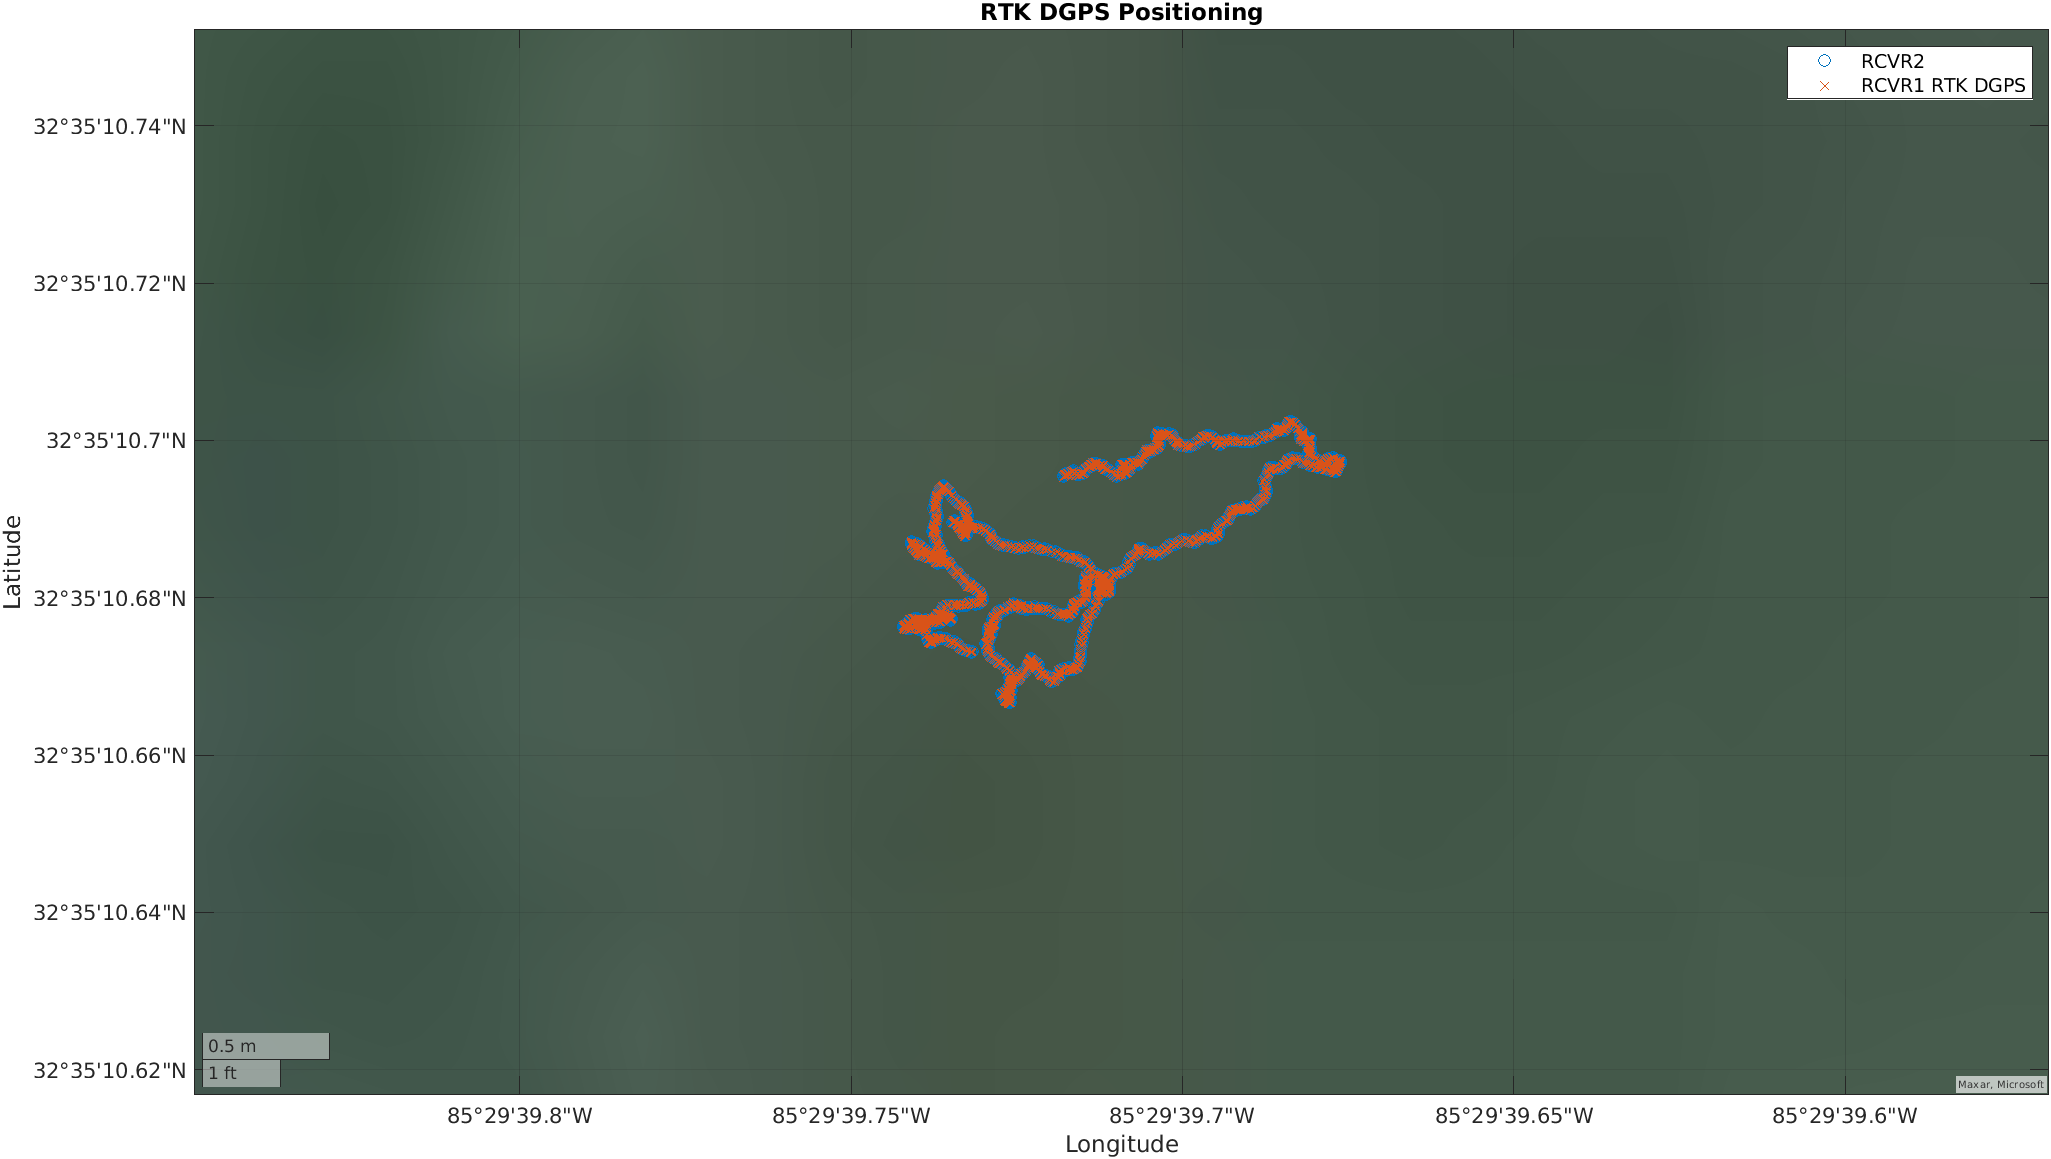
\includegraphics[width=0.85\textwidth]{p2_d.png}
      \caption{Static RTK DGPS Solution.}
    \end{figure}
    The statistics on the position difference between the receivers for each static DGPS 
    method are tabulated in \emph{Table 2} and shown in \emph{Figure 10}. These were taken 
    on the distance magnitude between the receivers.
    % \rowcolors{2}{white}{lightgray}
    \begin{table}[H]
      \centering
      \caption{Statistics for Static DGPS Position Difference.}
      \begin{tabular}{ P{5cm}|P{3cm} P{3cm} }
         & \boldmath$\mu (m)$ & \boldmath$\sigma (m)$ \\
         \hline
         \textbf{Reference} & \multicolumn{2}{c}{} \\
         L1 Position & 0.023808 & 0.012676 \\
         \hline
         \textbf{DGPS} & \multicolumn{2}{c}{} \\
         Psuedorange & 0.023808 & 0.012676 \\
         Carrier RTK & 0.000486 & 0.000309 \\
         \hline
         \textbf{Carrier Smoothing DGPS} & \multicolumn{2}{c}{} \\
         2 min & 0.010486 & 0.006701 \\
         8 min & 0.006056 & 0.003862 \\
         15 min & 0.006582 & 0.003554
      \end{tabular}
    \end{table}
    \begin{figure}[H]
      \centering
      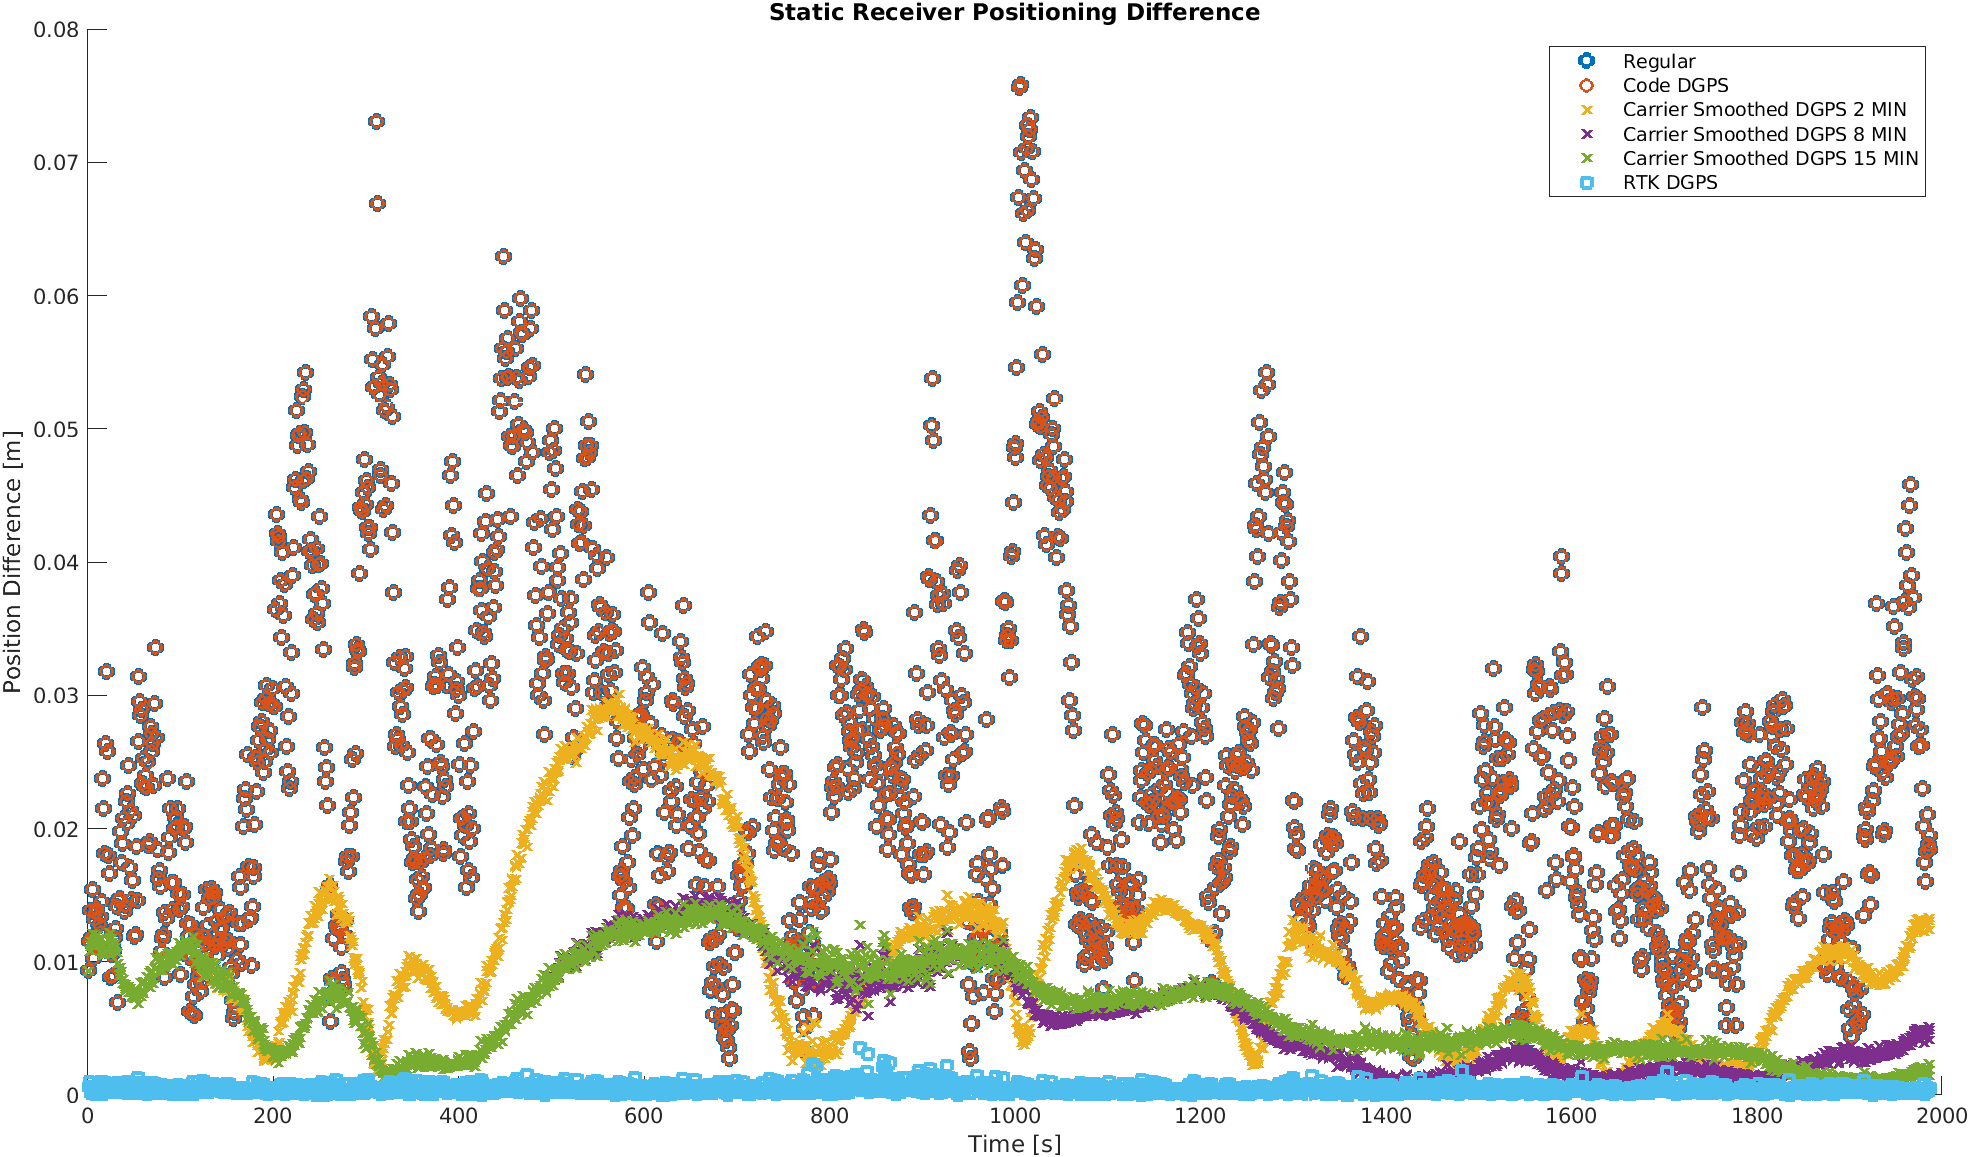
\includegraphics[width=0.85\textwidth]{p2_comp.png}
      \caption{DGPS Relative Position Vector Over Time.}
    \end{figure}
    As shown by the statistics, the RTK Positioning solution is by far the superior static 
    DGPS positioning method. This is due to the cleanliness of the carrier measurement 
    such that when using it to position provides an extremely clean solution with little 
    noise. The mean of this solution is less than $5(10^{-4})$ which is essentially $0$. 
    This carrier effect is also shown in the carrier smoothing technique as the carrier 
    greatly smooths out the psuedorange measurements leading their error to be reduced by 
    over 50\%. It is also apparent that the Code (psuedorange) DGPS solution is the exact 
    same as the independent receiver positioning. This is likely due to the receiver setup 
    as both are receiving measurements via the same antenna.
  
    \item \textbf{Dynamic Relative DGPS Positioning} \\
      The same DGPS solutions that were evaluated for two static receivers were then 
      performed with two dynamic receivers. This time however, each receiver had their own 
      antenna and had a static distance of 50 inches (1.27 meters) between them. Also note, 
      for the dynamic DGPS solutions, there were a few occurrences where both receivers did 
      not have a common 4 satellites in view, which were removed from the simulation. The 
      original GPS position solutions for both receivers were plotted against each other in 
      \emph{Figure 11}. The original GPS positions solutions were found using the least 
      squares method discussed in \emph{equation 1}. 
      \begin{figure}[H]
        \centering
        \begin{minipage}[b]{0.49\textwidth}
          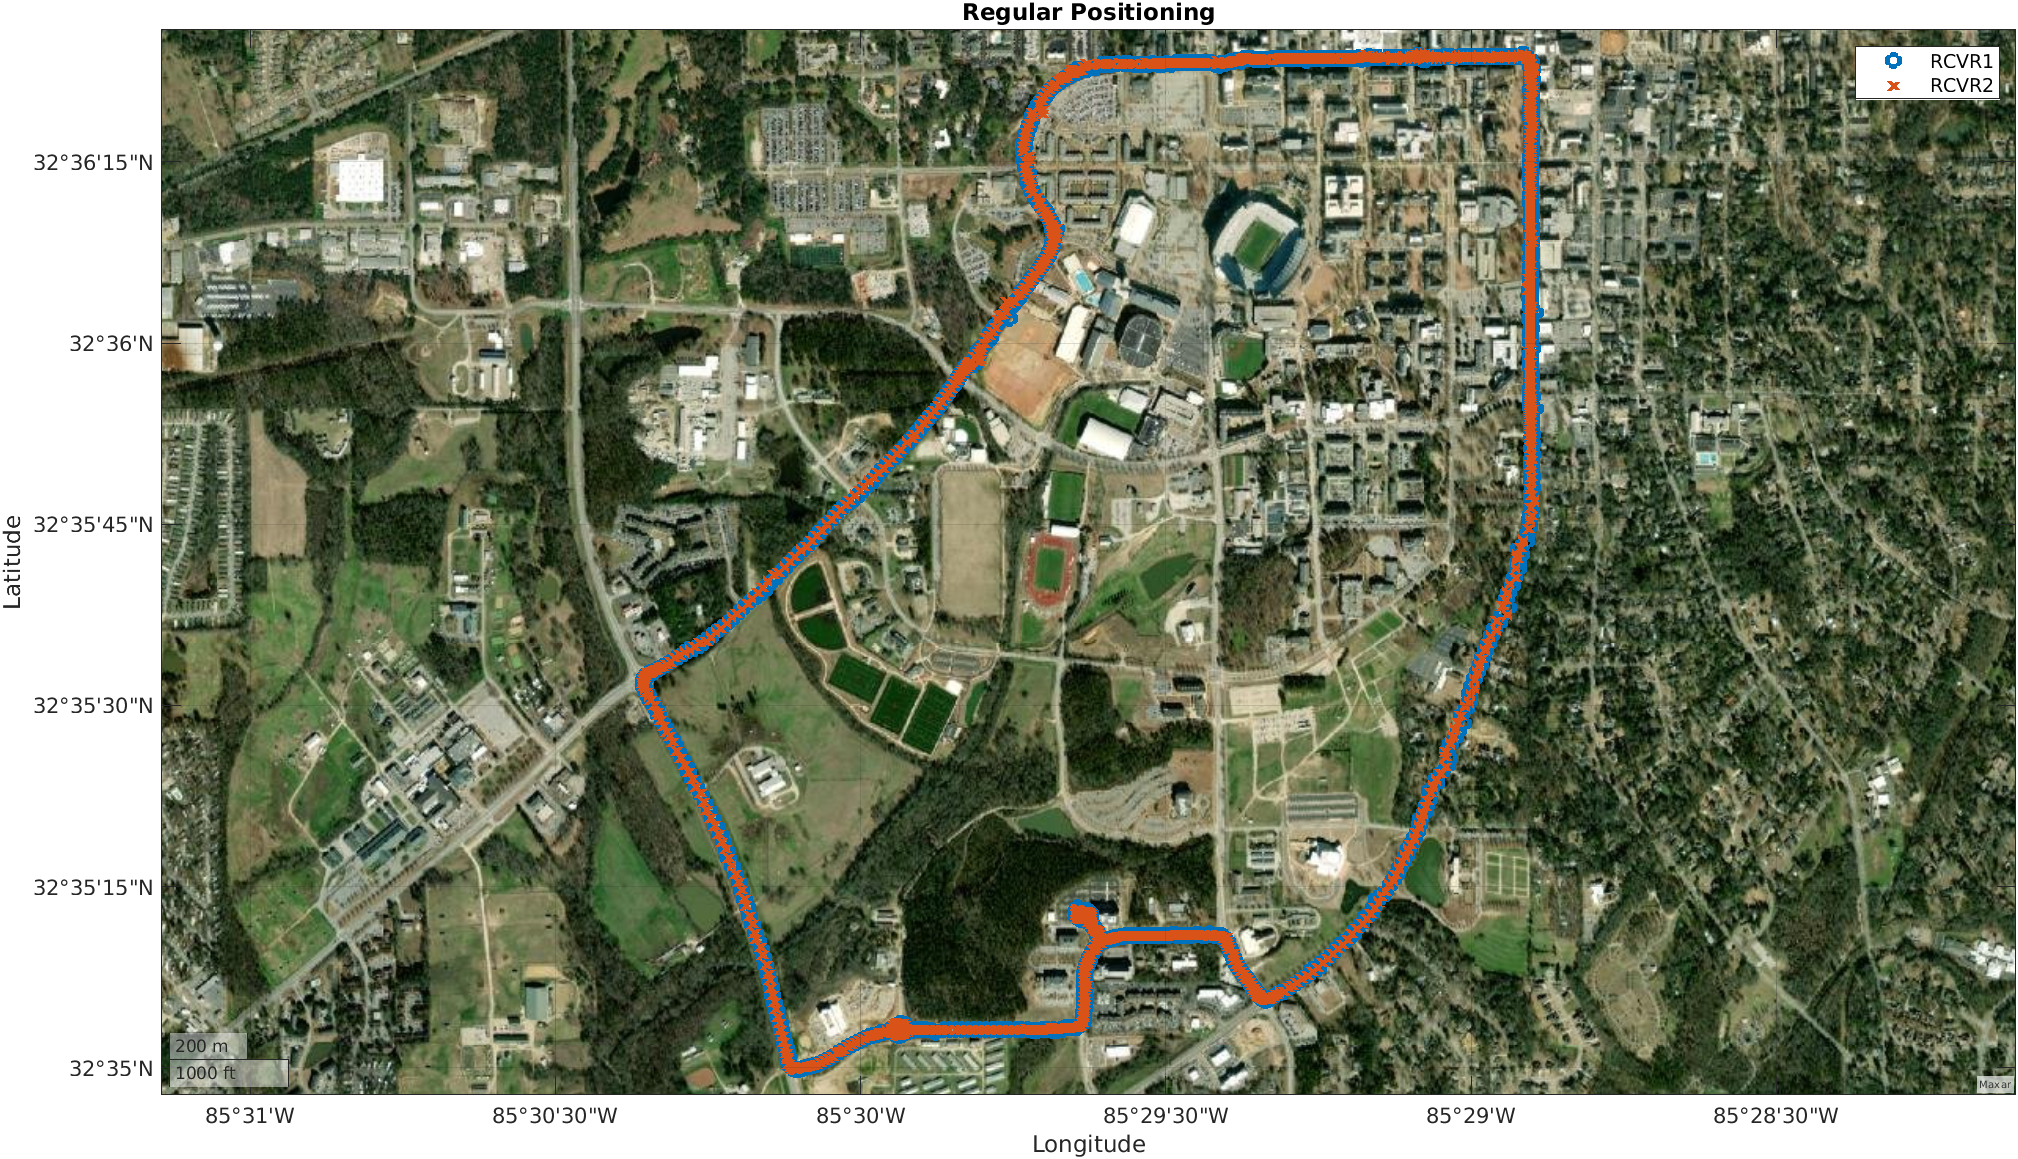
\includegraphics[width=\textwidth]{p3_a.png}
        \end{minipage}
        \begin{minipage}[b]{0.49\textwidth}
          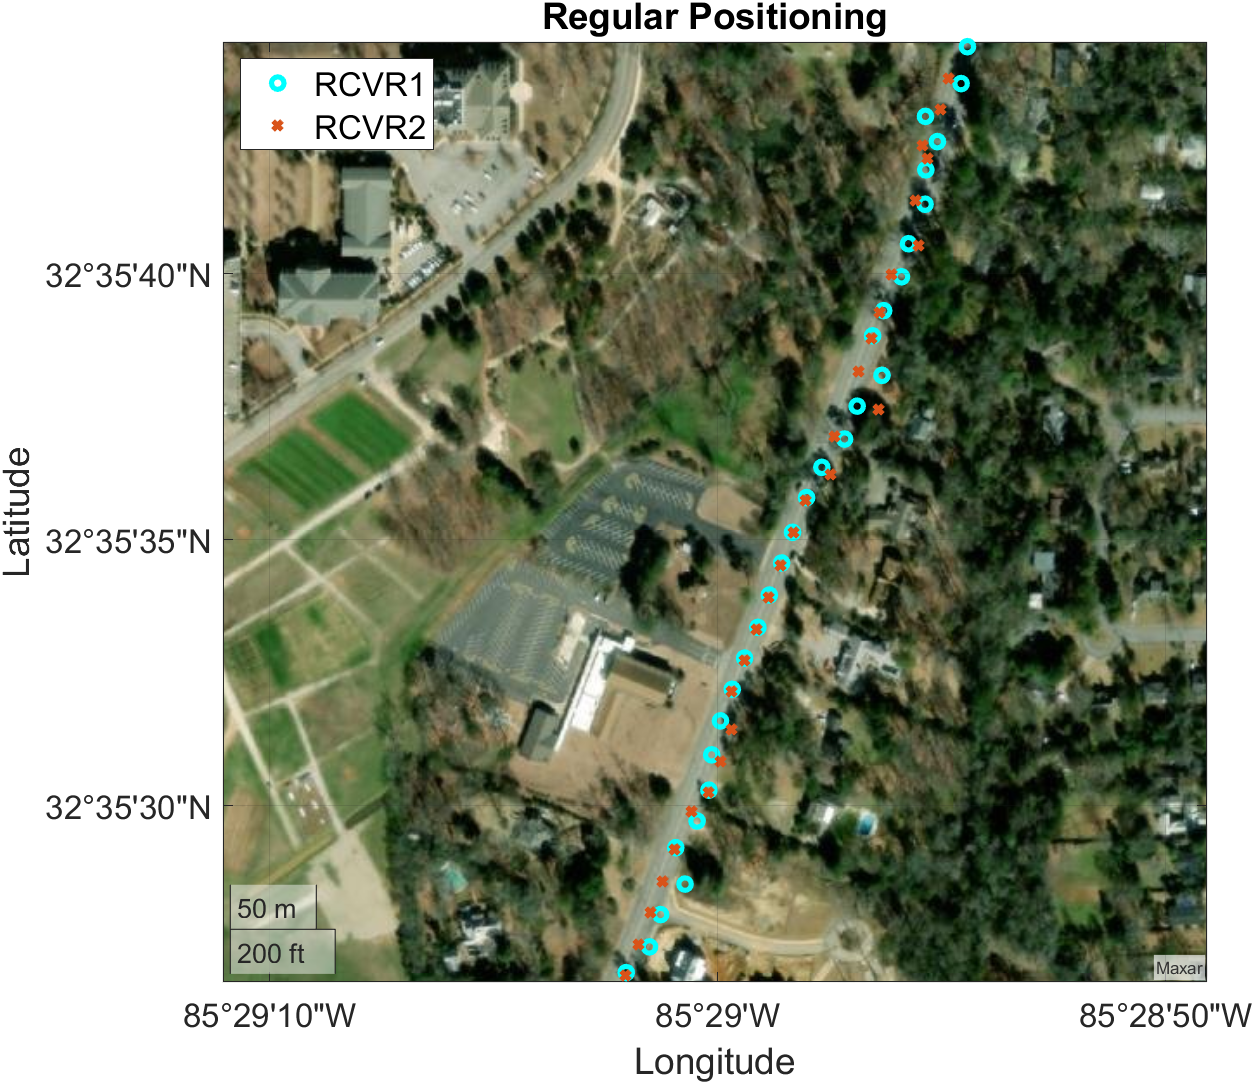
\includegraphics[width=\textwidth]{p3_a1.png}
        \end{minipage}
        \caption{Original Dynamic GPS Position Solutions.}
      \end{figure}
      Without using any form of DGPS the difference in position solutions between the two 
      receivers is somewhat large. The position difference between the two receivers should 
      only be 1.27 meters apart, but the mean position difference is over 7 meters. To 
      eliminate this error and variance different methods of DGPS positioning are performed 
      with the second receiver acting as the base. 
      \\ \\
      To start, code DGPS is performed using \emph{equation 5}. In addition to this, since 
      the distance between the receivers is static, the least squares solution for the 
      distance between the receivers was performed recursively to reduce spikes in error. 
      In recursive estimation, the covariance matrix is maintained across time epochs 
      leading to any new information being smoothed out by the uncertainty of prior 
      measurements along with the uncertainty of the new measurement. The position solution 
      for both code DGPS positions are shown on \emph{Figure 12} alongside the original 
      dynamic position solution.
      \begin{figure}[H]
        \centering
        \begin{minipage}[b]{0.49\textwidth}
          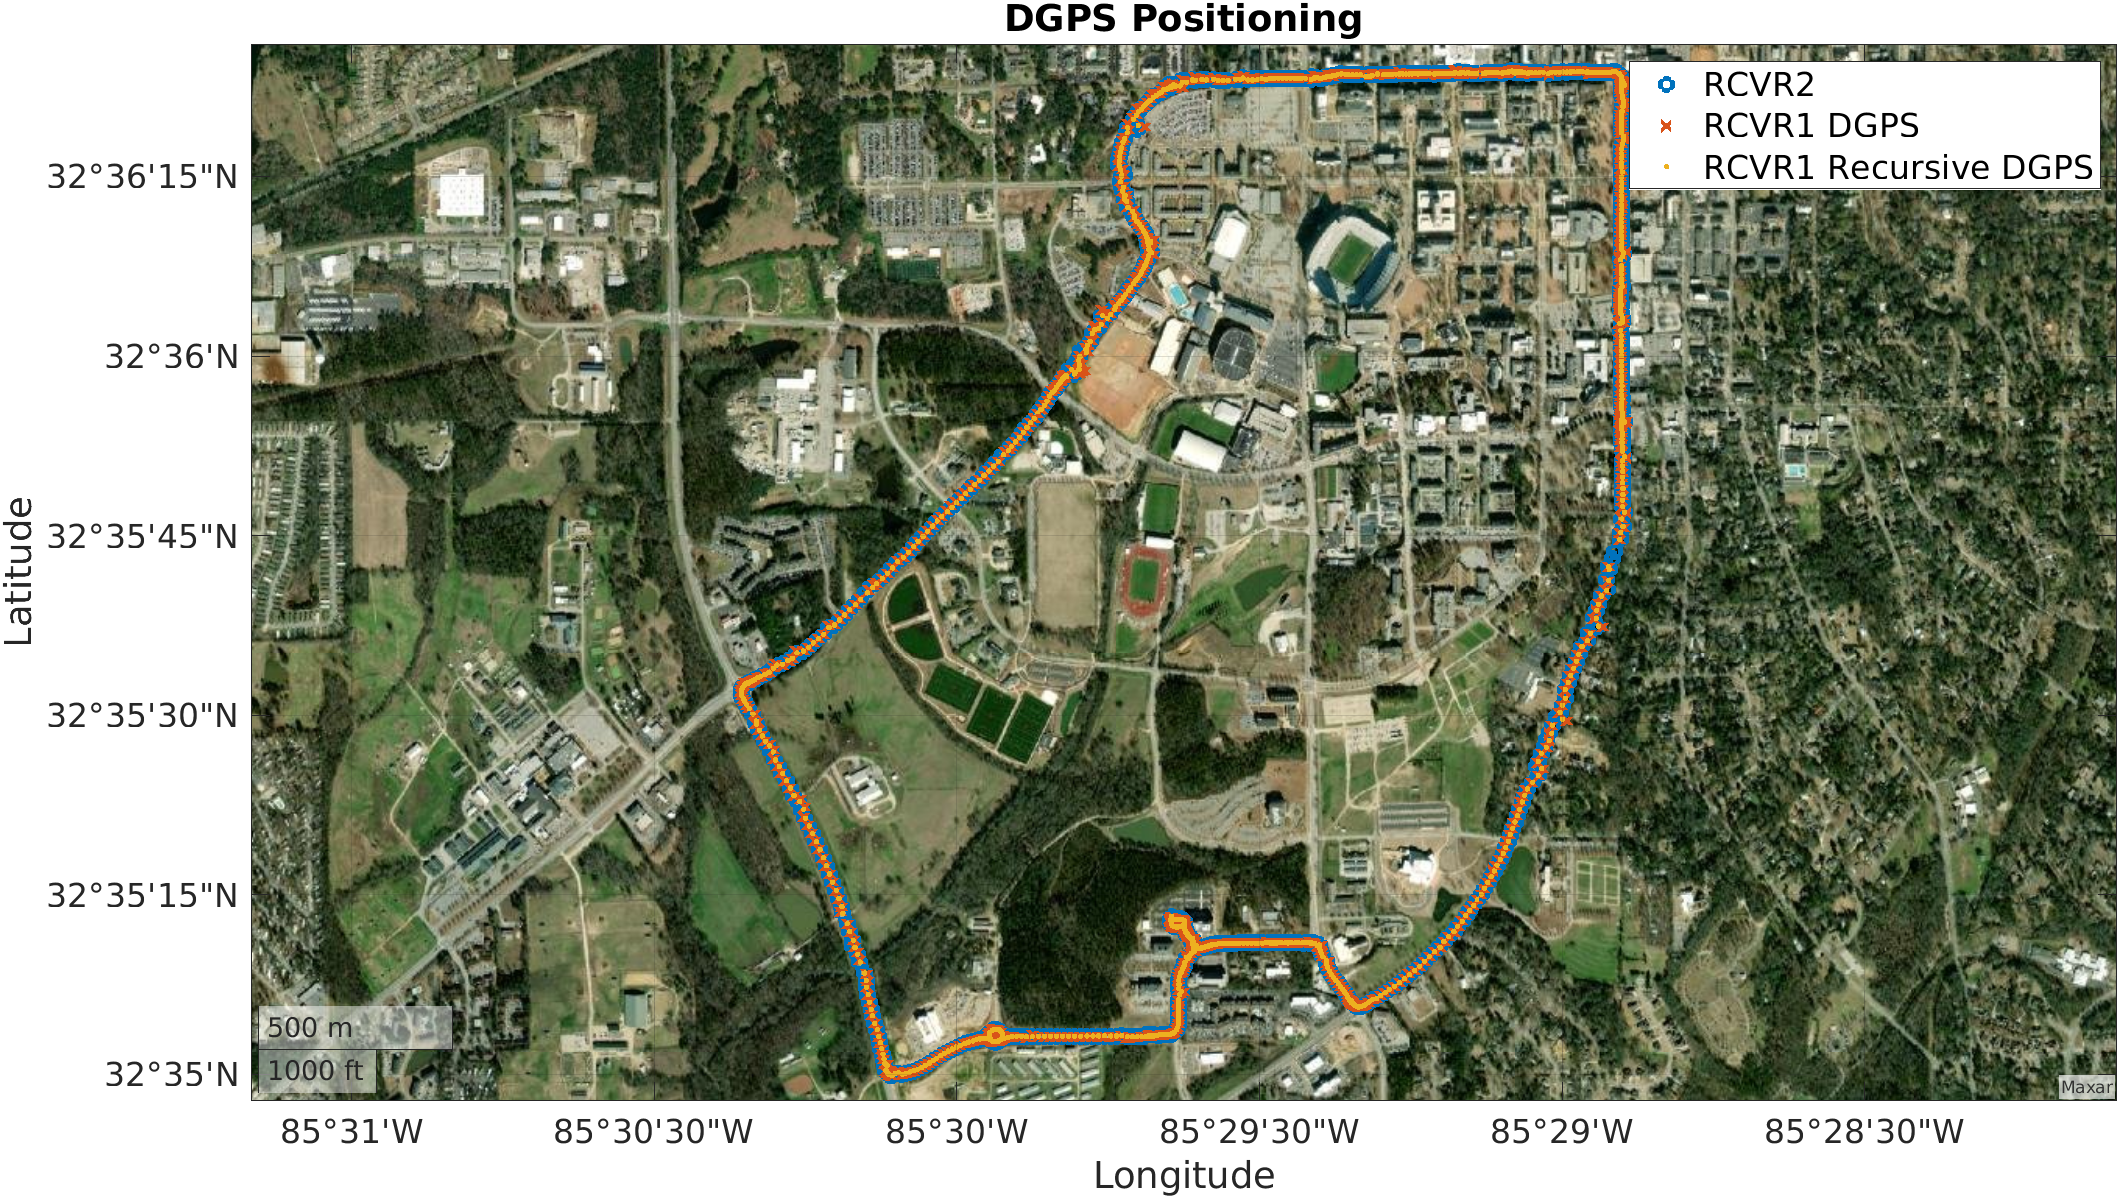
\includegraphics[width=\textwidth]{p3_b.png}
        \end{minipage}
        \begin{minipage}[b]{0.49\textwidth}
          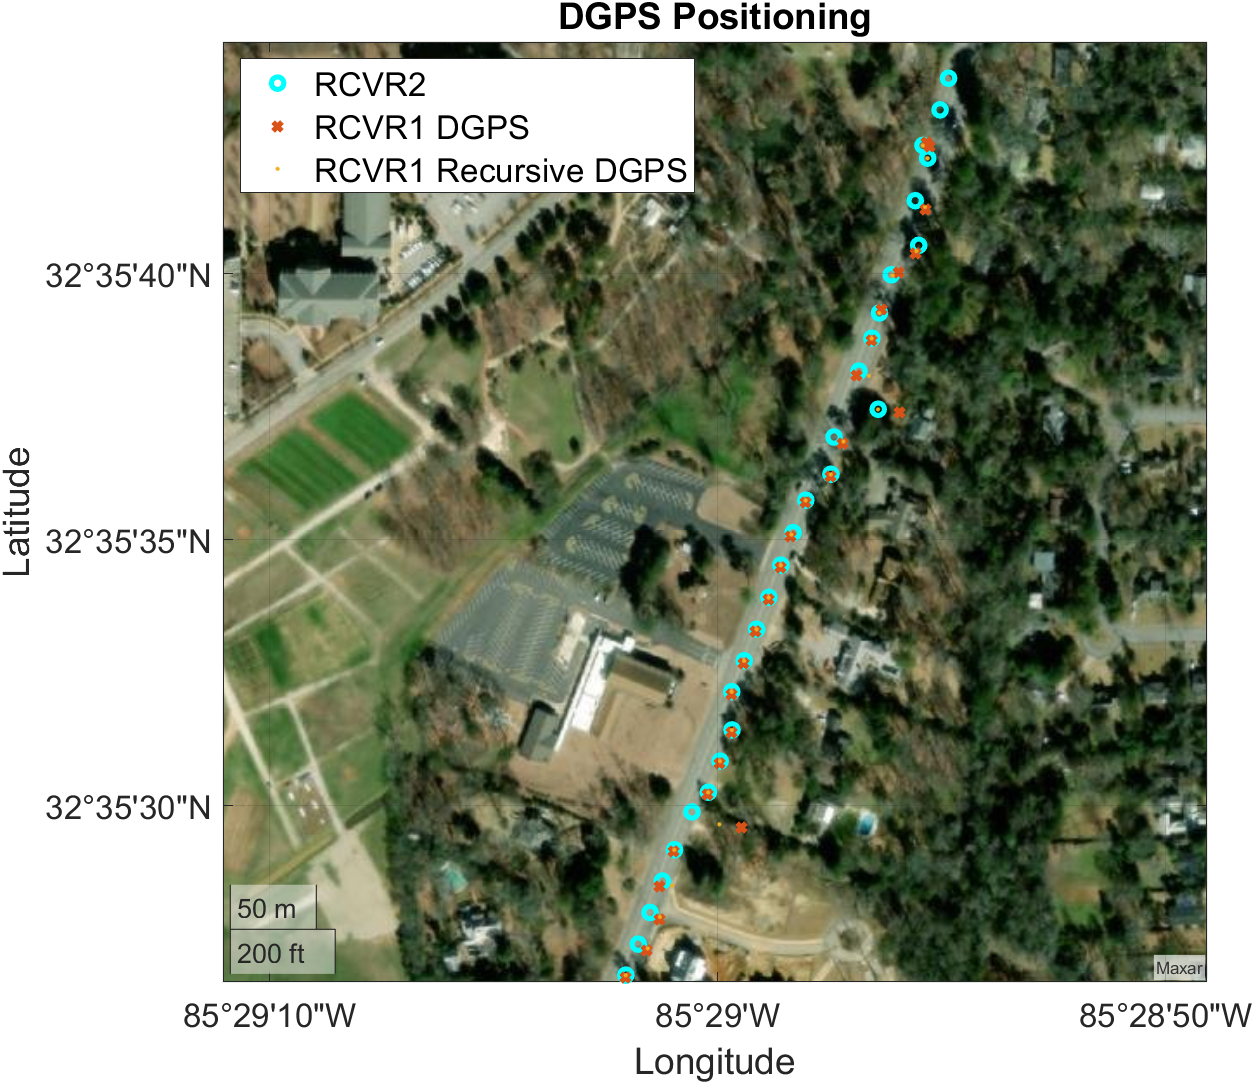
\includegraphics[width=\textwidth]{p3_b1.png}
        \end{minipage}
        \caption{Dynamic Code DGPS Position Solution.}
      \end{figure}
      Implementing code DGPS significantly decreases the difference between the receivers. 
      Any error due to the atmosphere are removed from the pseudorange measurements. 
      Additionally, recursive DGPS decreased the position error even more with a 1.6 meters 
      of position difference and a 0.4 meter standard deviation. Recursive estimation combats 
      areas of bad measurements by using the prior time epochs covariance matrix. 
      \\ \\
      Carrier phase smoothing DGPS was then performed on the dynamic data using 
      \emph{equation 6}. Averaging windows of 2, 8, and 15 minutes were evaluated as 
      potential time windows. Averaging was done with any satellite available for each time 
      step. Each satellite was individually smoothed while in view and smoothing was 
      restarted any time the satellite left view. \emph{Figure 13} gives the carrier phase 
      smoothing DGPS dynamic position solution plotted against the original position 
      solution.
      \begin{figure}[H]
        \centering
        \begin{minipage}[b]{0.49\textwidth}
          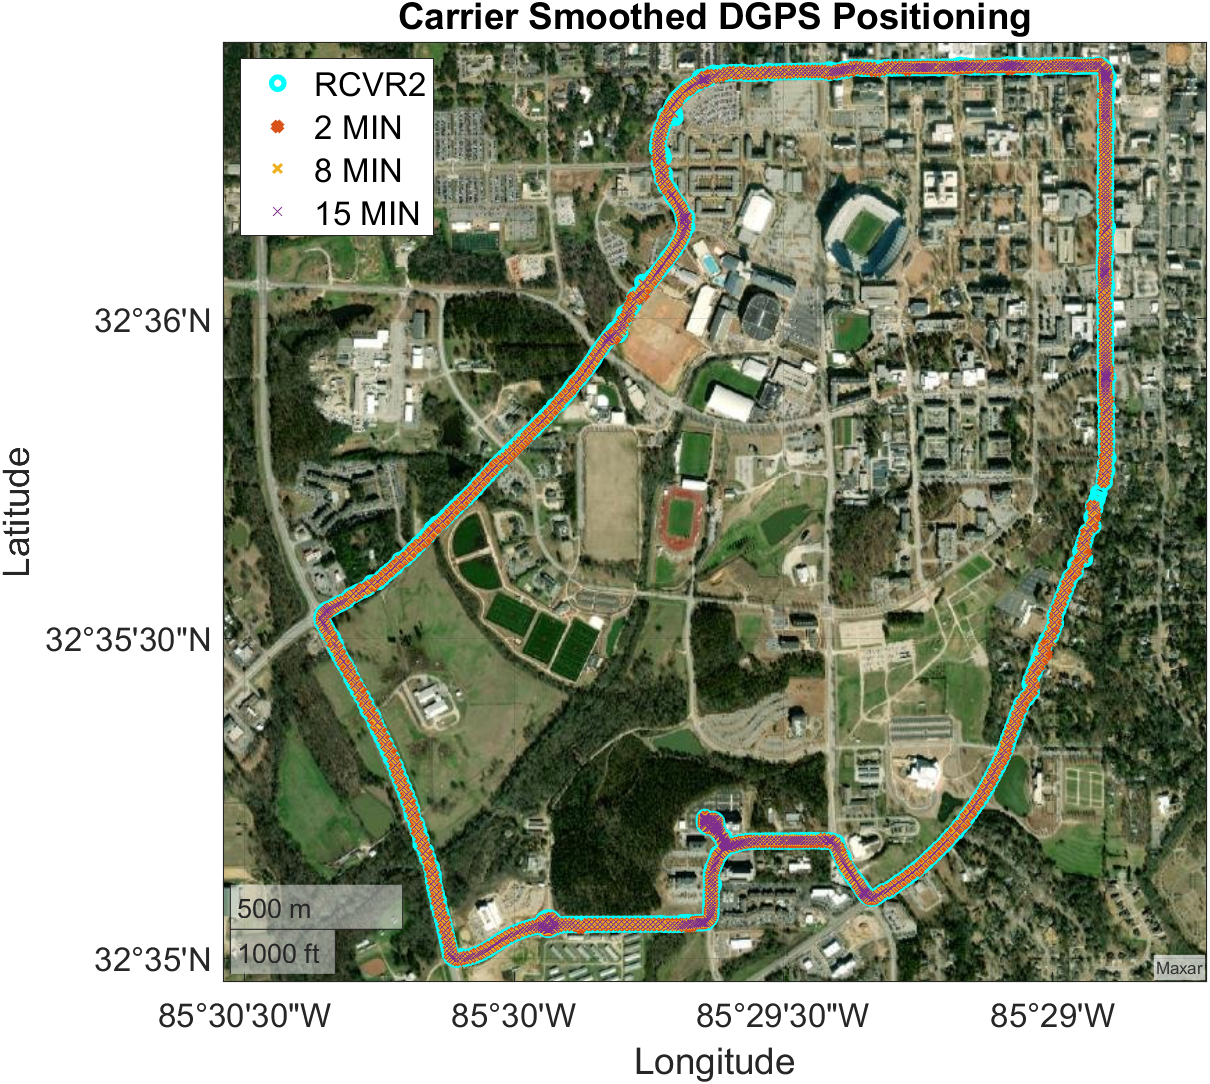
\includegraphics[width=\textwidth]{p3_c.png}
        \end{minipage}
        \begin{minipage}[b]{0.49\textwidth}
          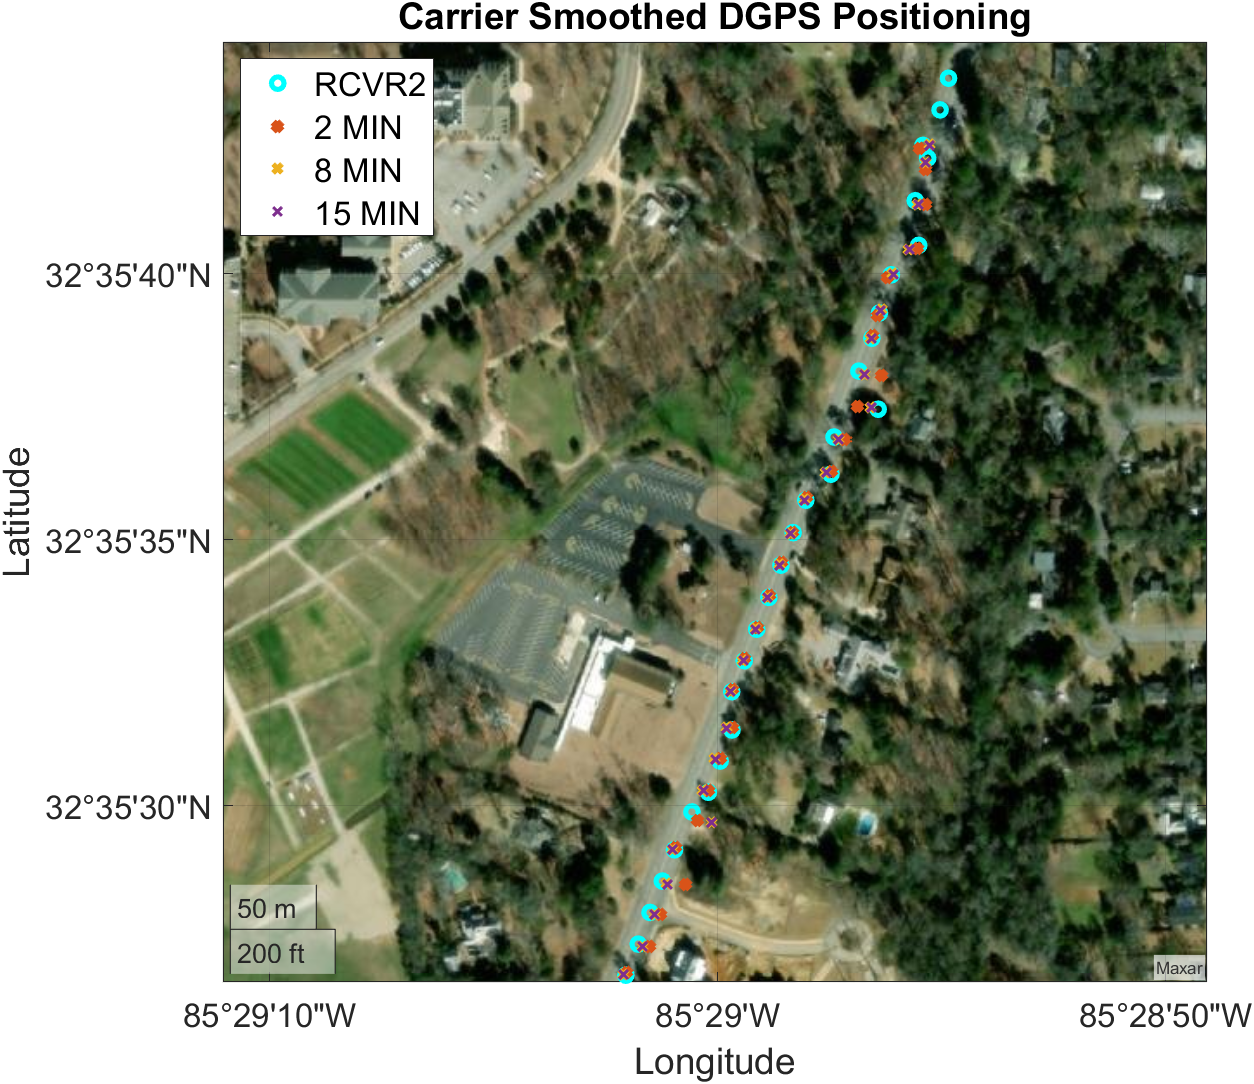
\includegraphics[width=\textwidth]{p3_c1.png}
        \end{minipage}
        \caption{Dynamic Carrier Phase Smoothed DGPS.}
      \end{figure}
      Each of the carrier phase smoothed DGPS position solutions decreased the amount of 
      range error in the measurements. Additionally, increasing the averaging window 
      decreased the amount of variance on the measurements. The 15 minute averaging 
      window never introduced a bias on the measurements, so it was the preferred averaging 
      window. Using the more precise carrier measurements mitigated the noise on the 
      pseudorange measurements. 
      \\ \\
      A RTK DGPS position was then computed using \emph{equations 7-9}. The integer 
      ambiguities were approximated using the Lambda method to increase fidelity. 
      \emph{Figure 14} gives the dynamic RTK DGPS position solution. Measurements were used 
      at time epochs where there were measurements available for both the L1 and L2 
      frequencies.
      \begin{figure}[H]
        \centering
        \begin{minipage}[b]{0.49\textwidth}
          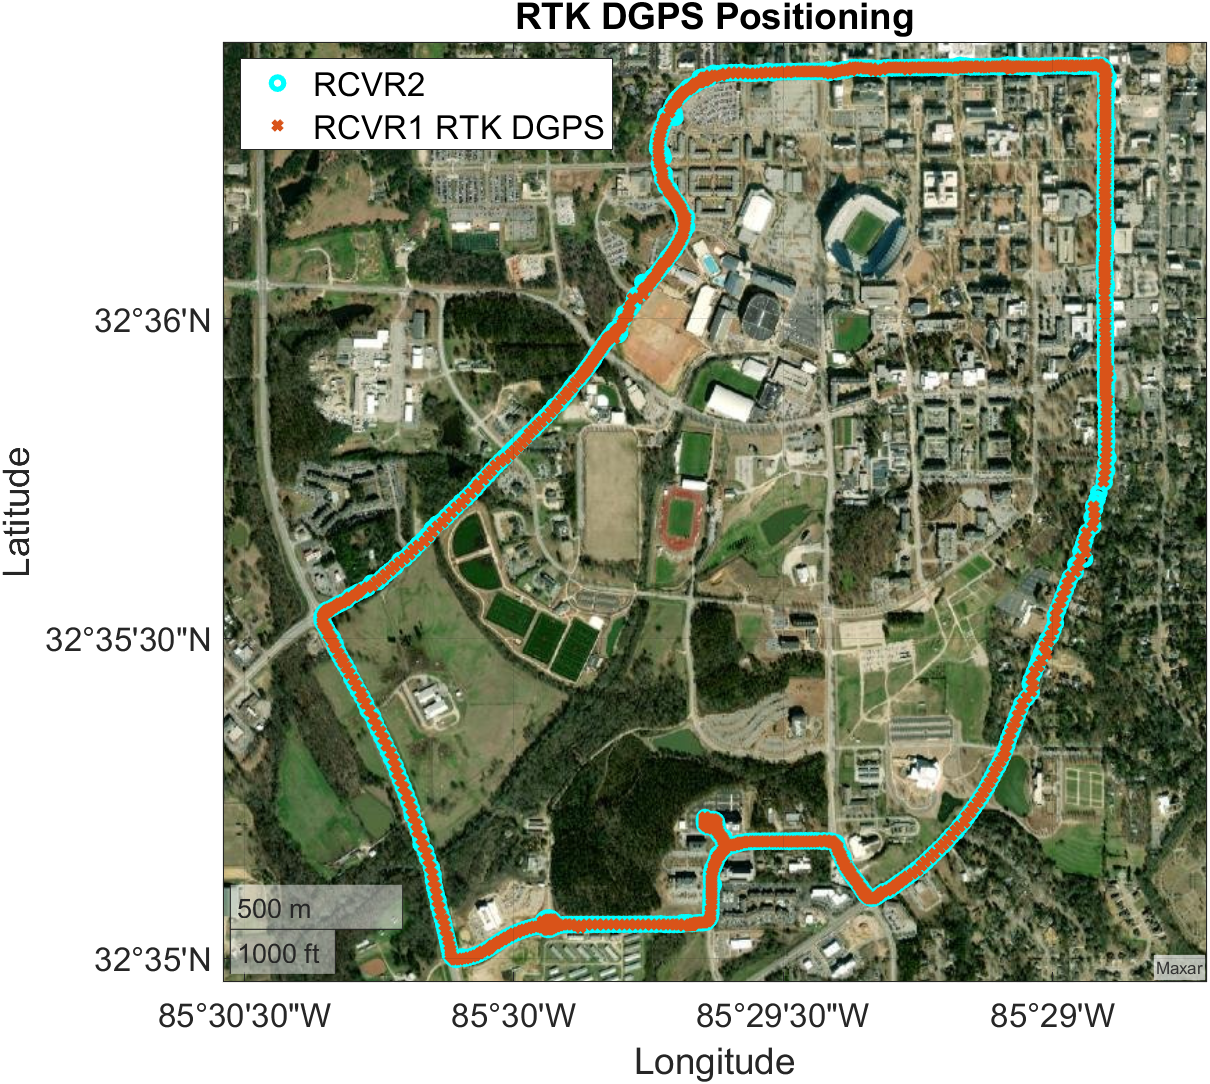
\includegraphics[width=\textwidth]{p3_d.png}
        \end{minipage}
        \begin{minipage}[b]{0.49\textwidth}
          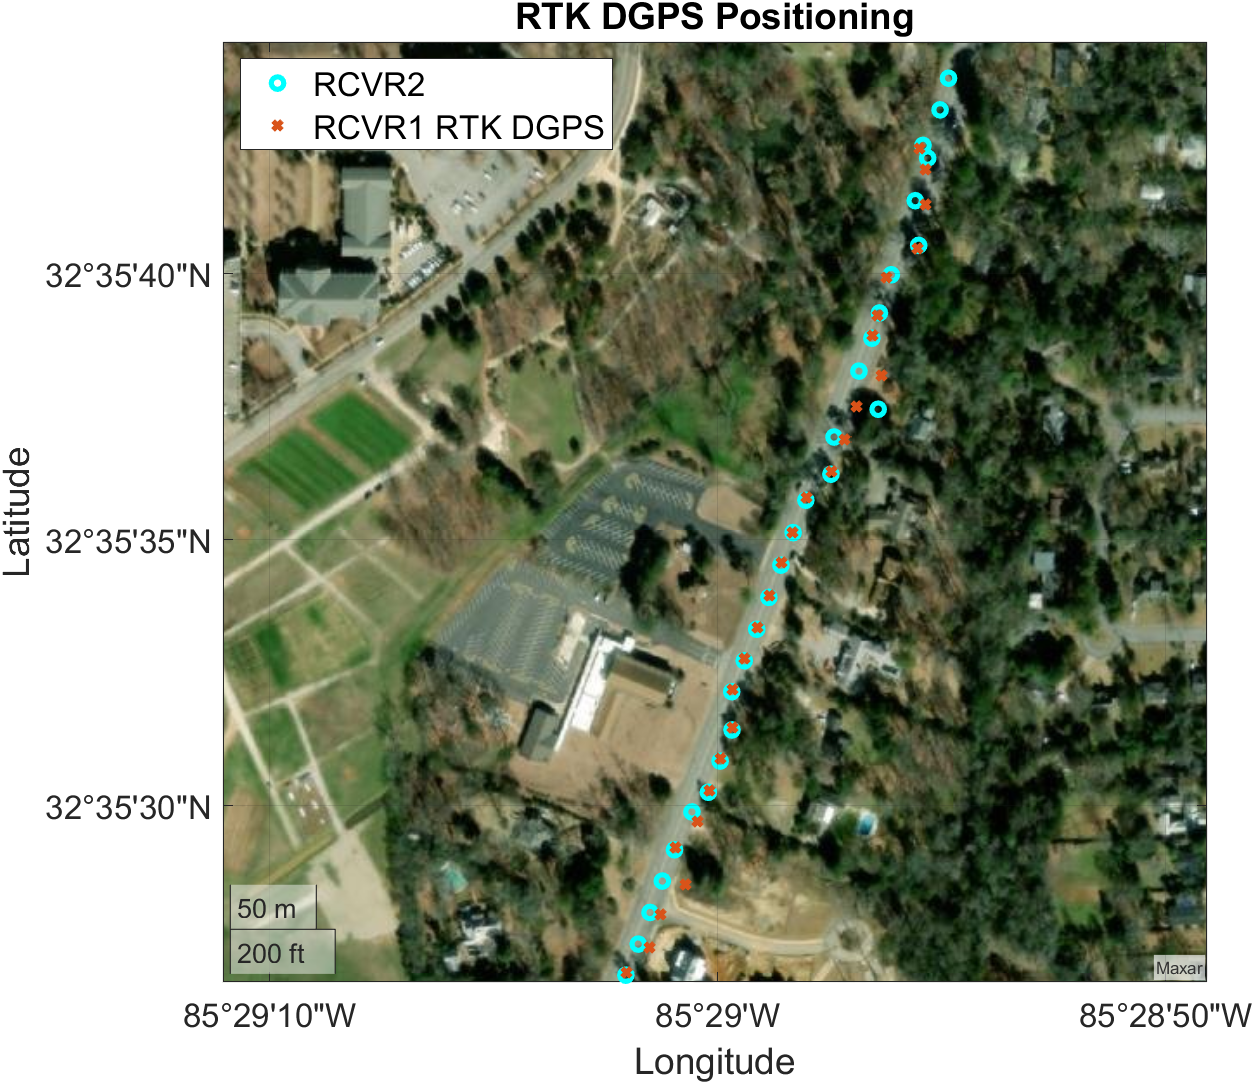
\includegraphics[width=\textwidth]{p3_d1.png}
        \end{minipage}
        \caption{Dynamic RTK DGPS.}
      \end{figure}
      The RTK DGPS solution improved the range error. Using the more precise carrier phase 
      measurement mitigates the noise on the measurements. Additionally, the DGPS removes 
      the atmospheric error. However, the RTK DGPS sometimes spikes in error. This is due to 
      the integer ambiguities being imprecise to measure when measurements are corrupted. 
      Additionally, some carrier phase measurements has to be thrown out when the difference 
      between measurements drastically increased. 
      \\ \\
      \emph{Figure 15} shows the range error for each DGPS method over time. \emph{Table 3} 
      shows the mean and standard deviation of the ranging errors for each DGPS position 
      solution.
      % \rowcolors{2}{white}{lightgray}
      \begin{table}[H]
        \centering
        \caption{Statistics for Static DGPS Position Difference.}
        \begin{tabular}{ P{5cm}|P{3cm} P{3cm} }
          & \boldmath$\mu (m)$ & \boldmath$\sigma (m)$ \\
          \hline
          \textbf{Reference} & \multicolumn{2}{c}{} \\
          L1 Position & 6.476002 & 7.177811 \\
          \hline
          \textbf{DGPS} & \multicolumn{2}{c}{} \\
          Psuedorange & 4.452806 & 4.452806 \\
          Recursive & 1.627683 & 0.413855 \\
          Carrier RTK & 4.452835 & 4.755819 \\
          \hline
          \textbf{Carrier Smoothing DGPS} & \multicolumn{2}{c}{} \\
          2 min & 4.452806 & 4.750667 \\
          8 min & 3.941766 & 3.114561 \\
          15 min & 3.361717 & 2.972168
        \end{tabular}
      \end{table}
      \begin{figure}[H]
          \centering
          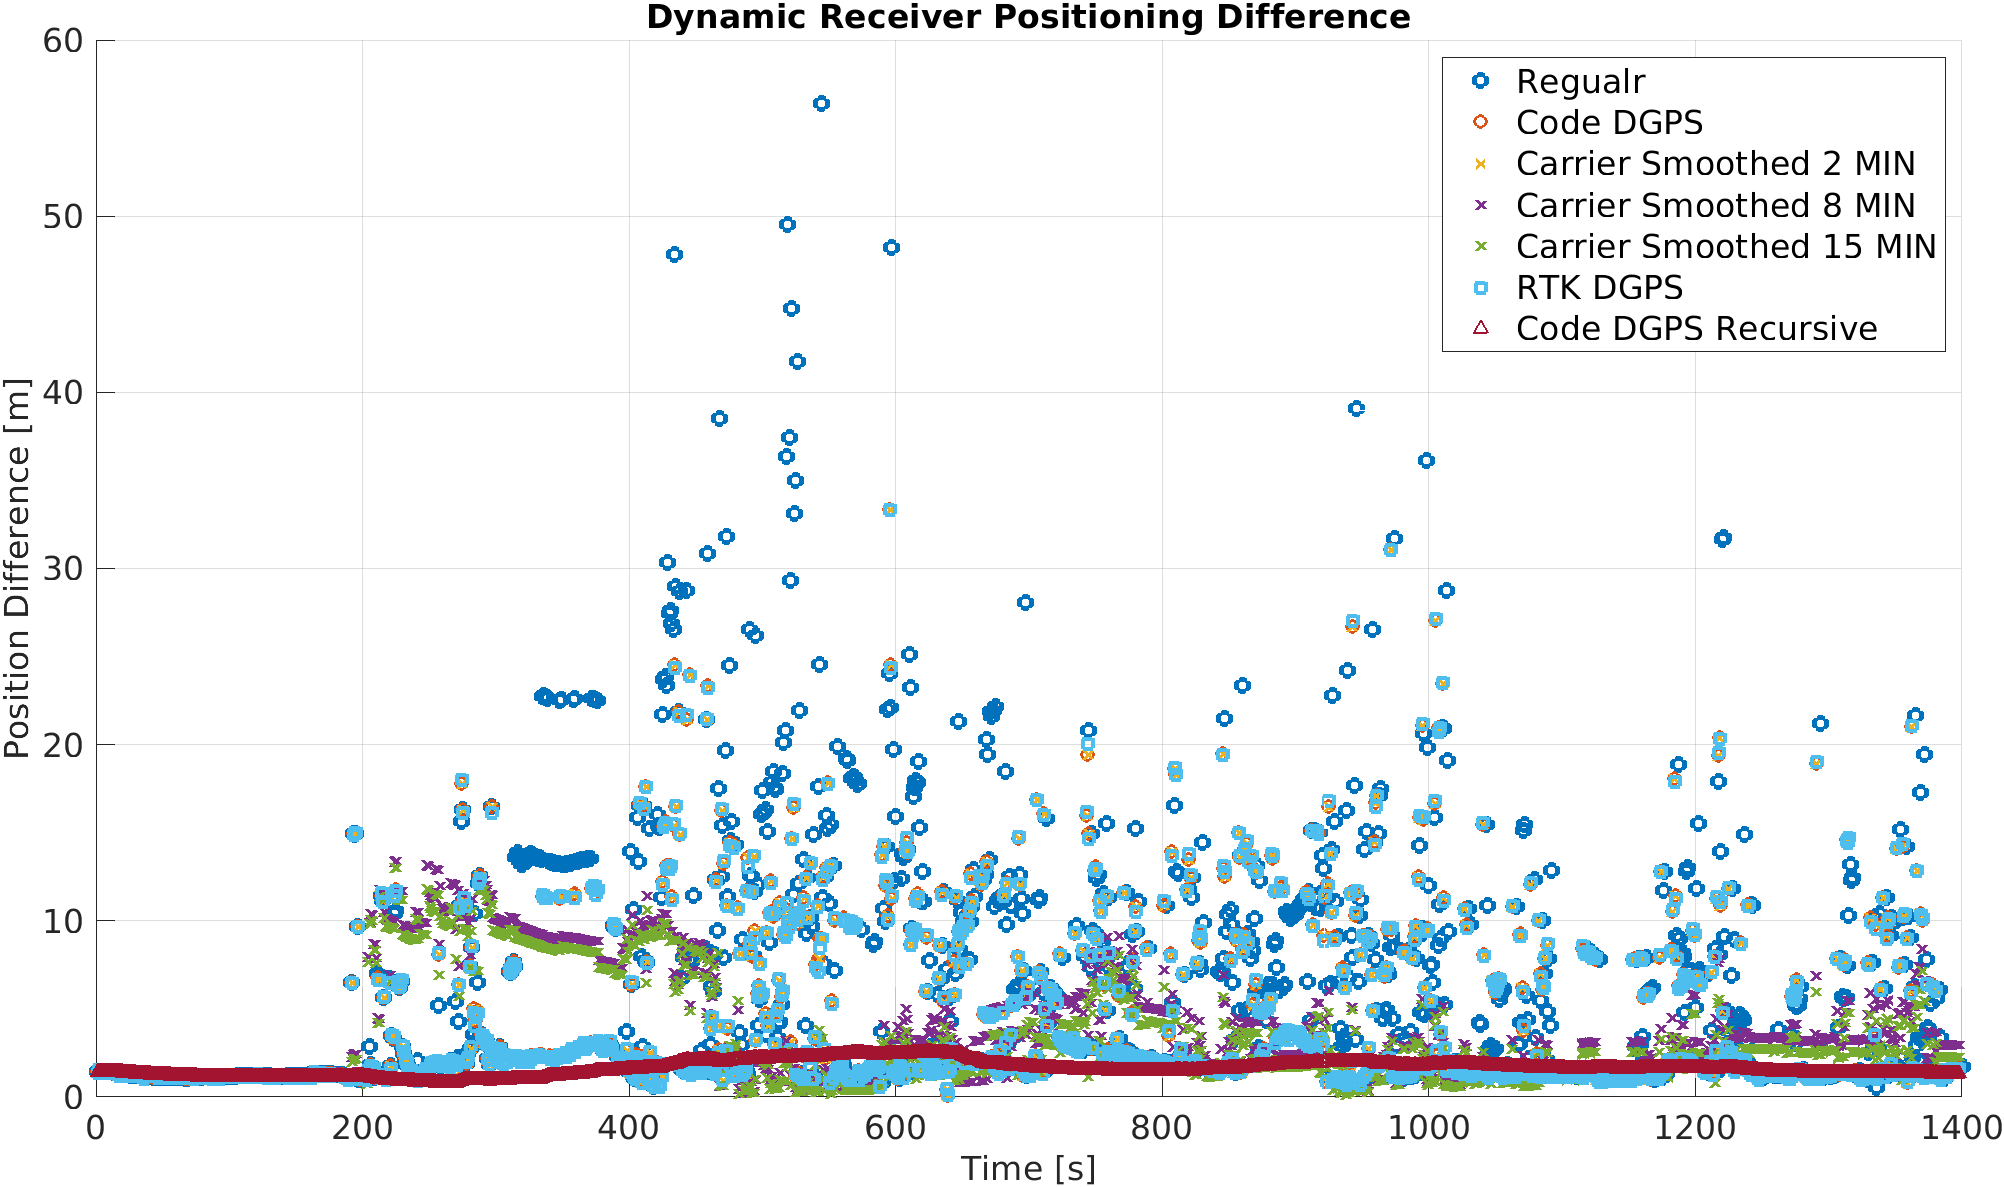
\includegraphics[width=0.85\textwidth]{p3_comp.png}
          \caption{Range Error Comparison of Dynamic DGPS.}
      \end{figure}
      From the figure and table it is shown that the recursive code DGPS is the optimal 
      method or error mitigation for the dynamic data set. It had the lowest mean range 
      error, and also displayed the least amount of variance. DGPS eliminates the atmospheric 
      error while the recursive elements smooth the results since the distance between the 
      receivers should remain constant. The 8 and 15 minute carrier 
      smoothing position solution also gave solutions with low range error and variance. The 
      cleaner carrier phase measurements helped to control the noise on the pseudorange 
      measurements while also getting the added effects if DGPS. While every method reduced 
      the range error, the normal code DGPS, RTK DGPS, and 2 minute carrier smoothed solution 
      experienced considerable variance. In each of these methods, there was no control on 
      the noise of the measurements. Since the data was taken while moving, the quality of 
      the measurements was inherently worse. It should also be noted that the integer 
      ambiguity estimated for the RTK DGPS solution was sporadic due to poor quality 
      measurements. 
      \\ \\
      DGPS was also used to deduce the vehicle attitude during the run. The equation to 
      solve for the azimuth using DGPS is given as:
      \begin{equation}
        \psi=tan^{-1}\left({\dfrac{\delta E}{\delta N}}\right)
      \end{equation}
      where $\psi$ is the azimuth, $\delta E$ is the east distance between the two receivers, 
      and $\delta N$ is the north distance between the two receivers. The distance between 
      the two receivers is the calculated relative position vector using the recursive code 
      DGPS. This DGPS solution method was used because it displayed the most accurate results 
      for the dynamic scenario. The calculated azimuth was plotted against the GPS course 
      derived from GPS velocity given in \emph{equation 11} in \emph{figure 16}. To match 
      the frames as closely as possible, the azimuth was rotated by 15 degrees.
      \begin{figure}[H]
        \centering
        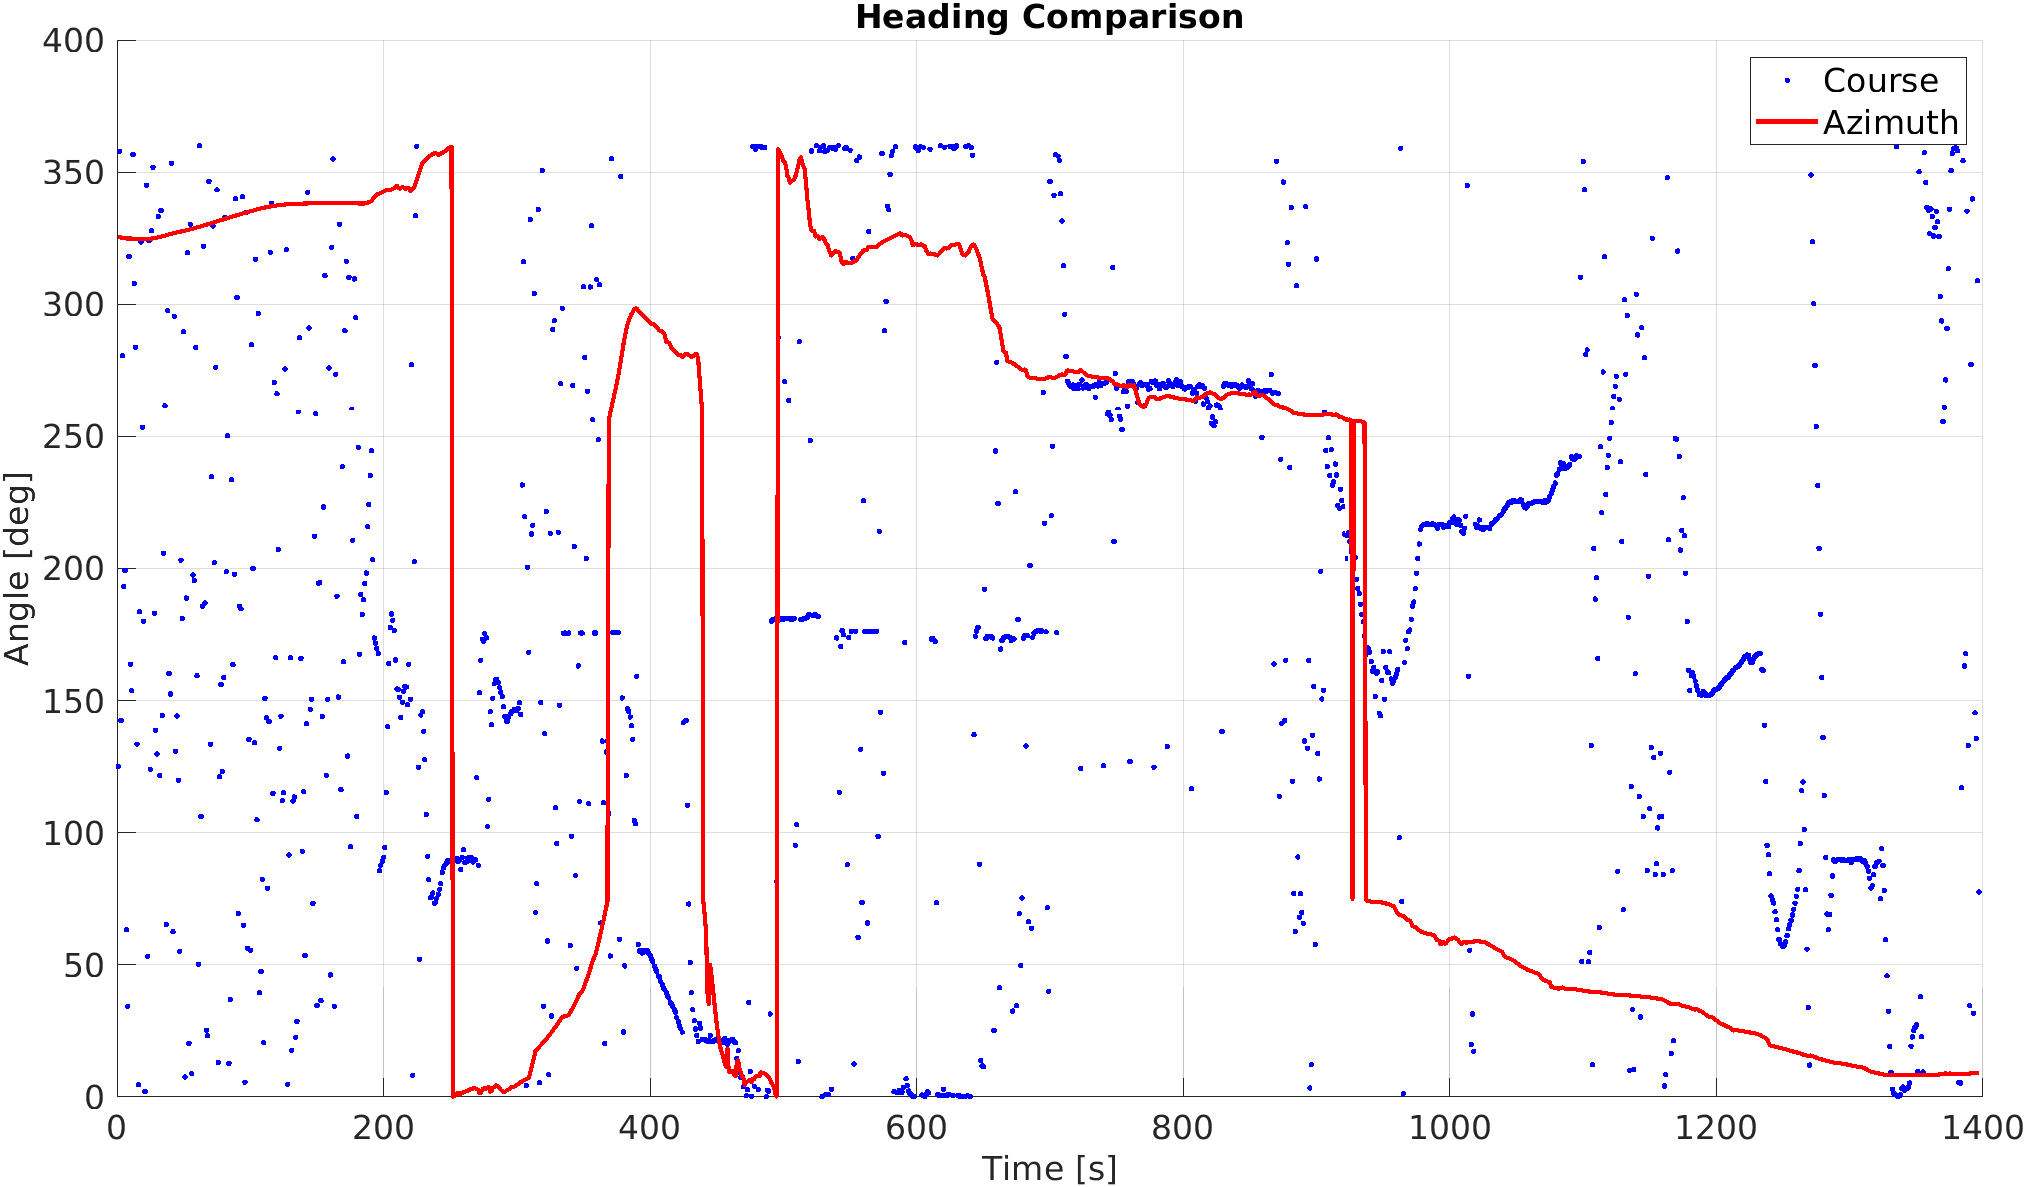
\includegraphics[width=0.85\textwidth]{p3_e.png}
        \caption{Azimuth vs GPS Course.}
      \end{figure}
      \begin{equation}
        \psi=tan^{-1}\left({\dfrac{\dot{E}}{\dot{N}}}\right)
      \end{equation}
      The calculated azimuth roughly matches the GPS course. While the trends are the same, 
      the exact values do no always line up. The bias and variance on the DGPS solution 
      certainly account for some of this error. The course measurements are also heavily 
      predicated on the raw measurements of the base receiver. Corrupted measurements could 
      greatly effect the course solution. Stopped motion also hurts the comparison, as the 
      calculated azimuth will yield results while the GPS course will not. This is due to 
      the GPS course being calculated based on velocity.
    
    \item \textbf{LAAS DGPS Positioning} \\
      In this section, the same DGPS solution techniques explored in previous parts were 
      used, but in a more practical scenario. The position solution for a dynamic receiver 
      is calculated using a static receiver as a base. To start, GPS position solutions were 
      determined for both the static and dynamic receiver. This was done using the least 
      squares method discussed in \emph{equation 1}. \emph{Figure 17} shows the standalone 
      position solutions for both receivers. It is important to note that the receiver 
      measurements were time synced using GPS time. 
      \begin{figure}[H]
        \centering
        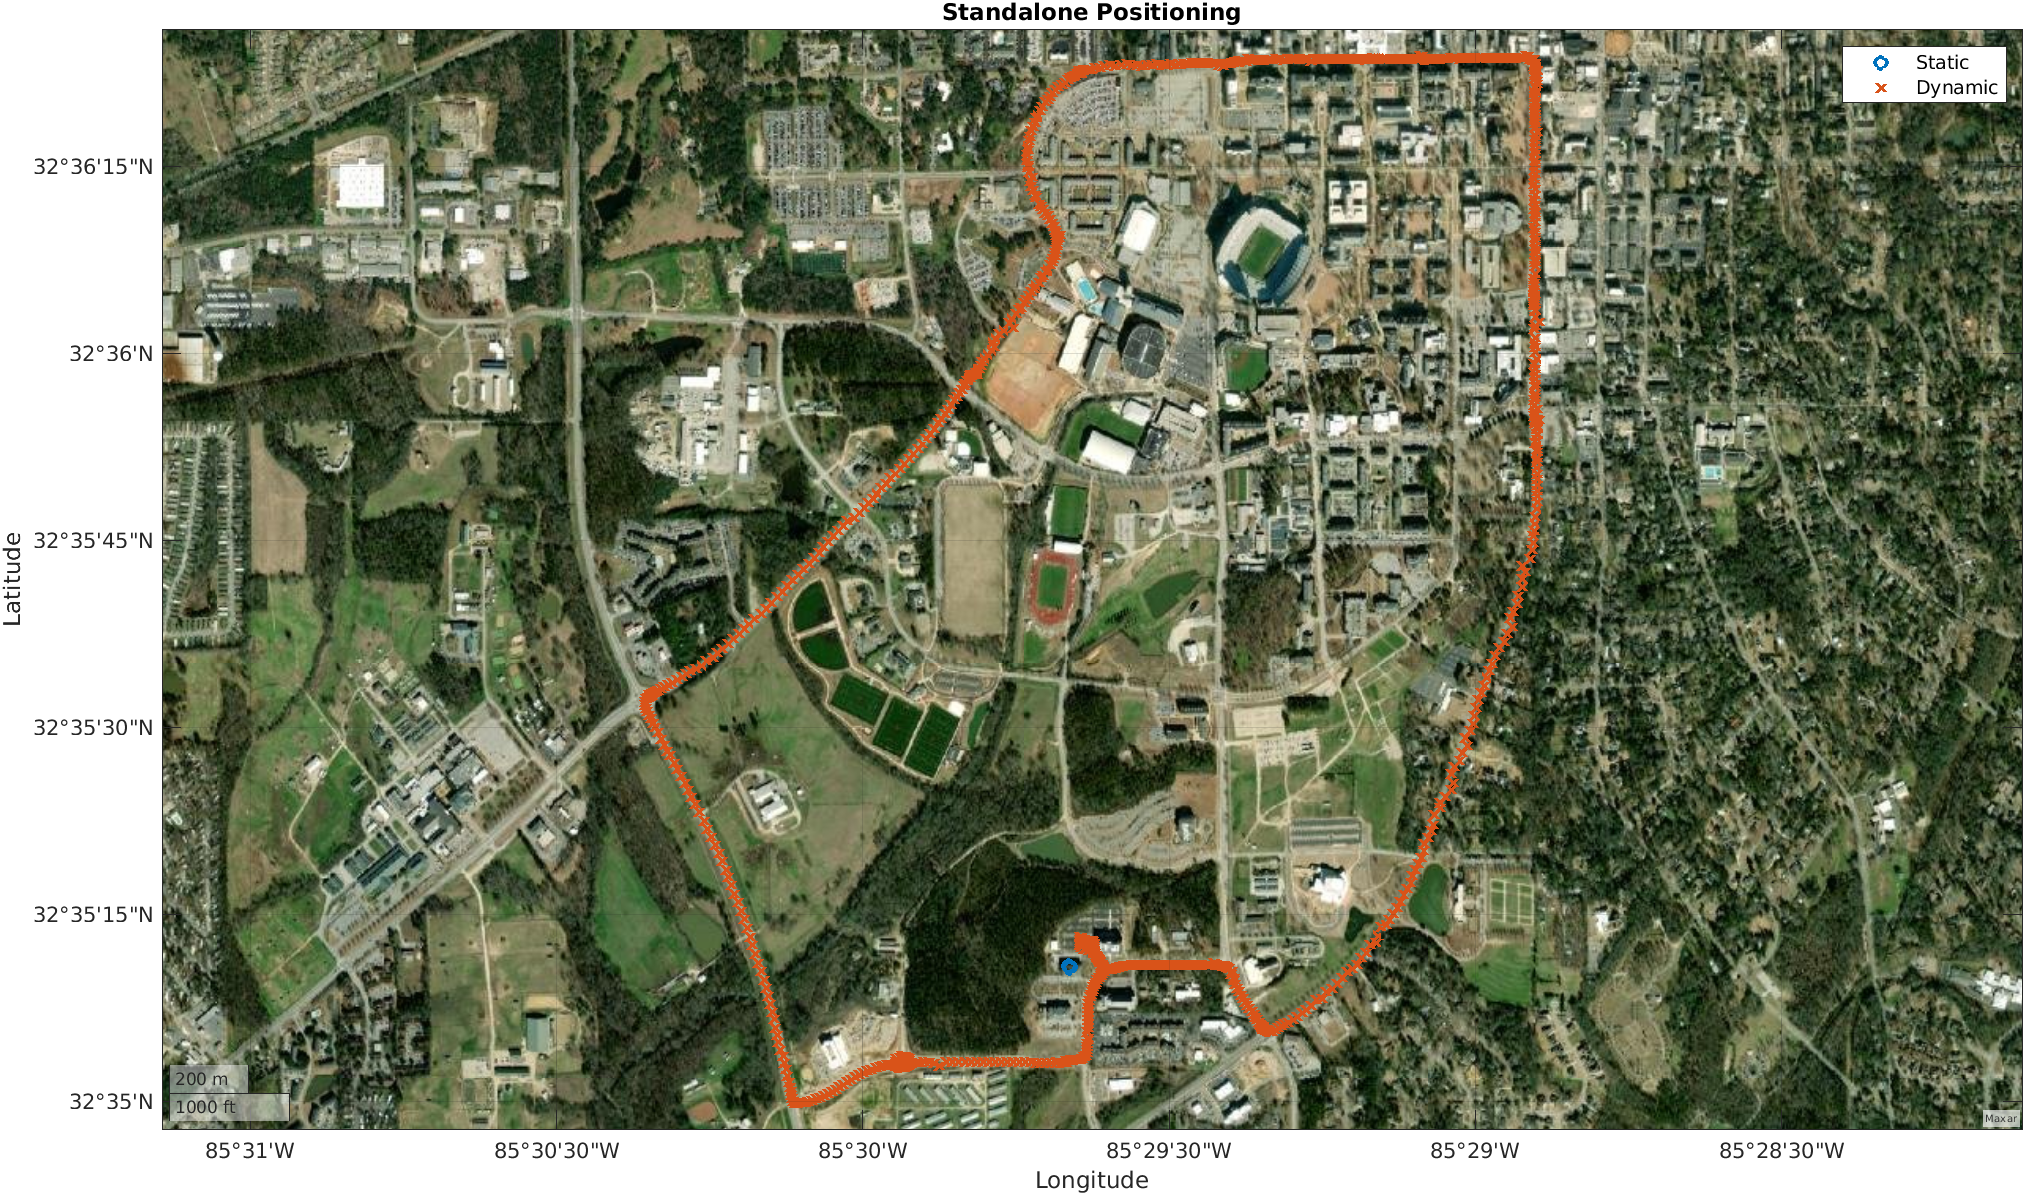
\includegraphics[width=0.85\textwidth]{p4_a.png}
        \caption{Standalone GPS Positioning Solutions.}
      \end{figure}
      From \emph{Figure 18} it can be seen that the static data was taken at the Auburn MRI 
      building while the dynamic data was taken on a path around Auburn's campus. Code DGPS 
      was then performed between the dynamic and static receivers using \emph{equation 5}. 
      The position solution for this code DGPS is shown on \emph{Figure 18}. Additionally, 
      \emph{Figure 19} gives the ECEF difference over time between the original and code 
      DGPS dynamic position solutions. 
      \begin{figure}[H]
        \centering
        \begin{minipage}[b]{0.49\textwidth}
          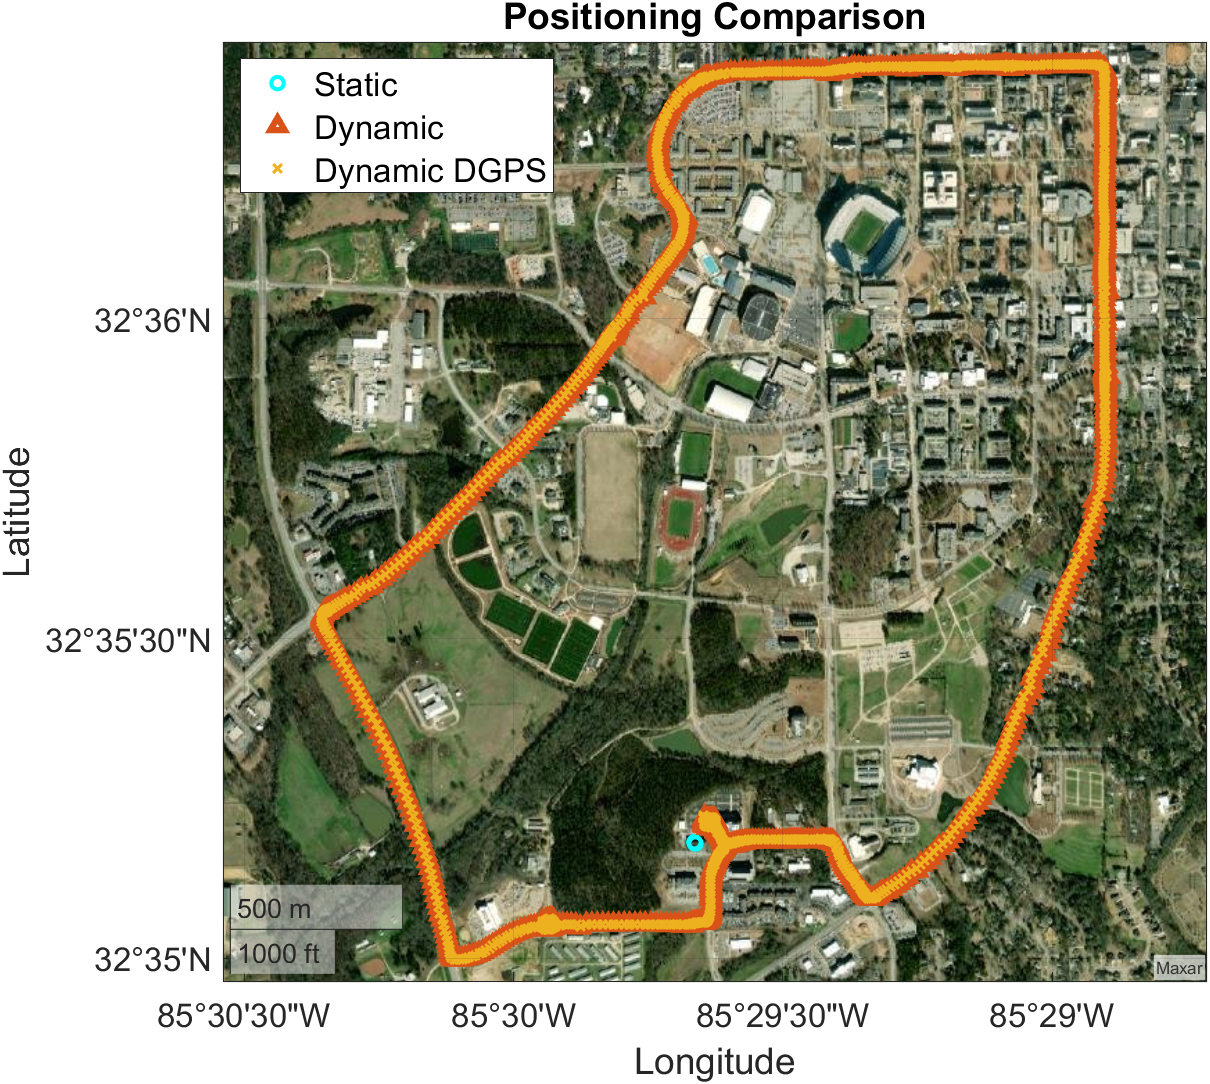
\includegraphics[width=\textwidth]{p4_comp.png}
        \end{minipage}
        \begin{minipage}[b]{0.49\textwidth}
          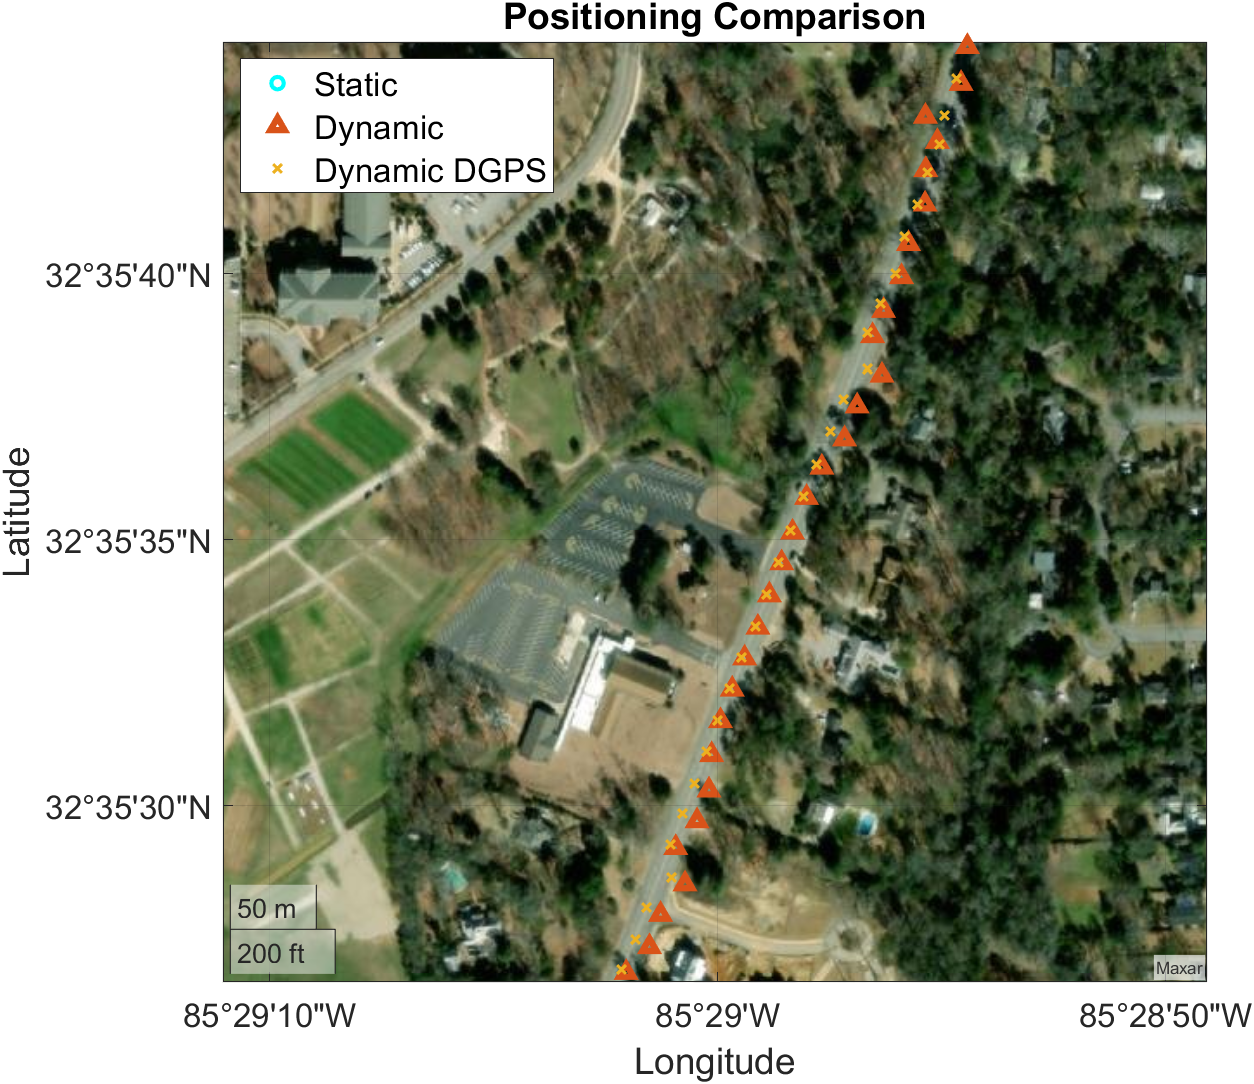
\includegraphics[width=\textwidth]{p4_comp2.png}
        \end{minipage}
        \caption{ECEF Position Difference Over Time.}
      \end{figure}
      \begin{figure}[H]
        \centering
        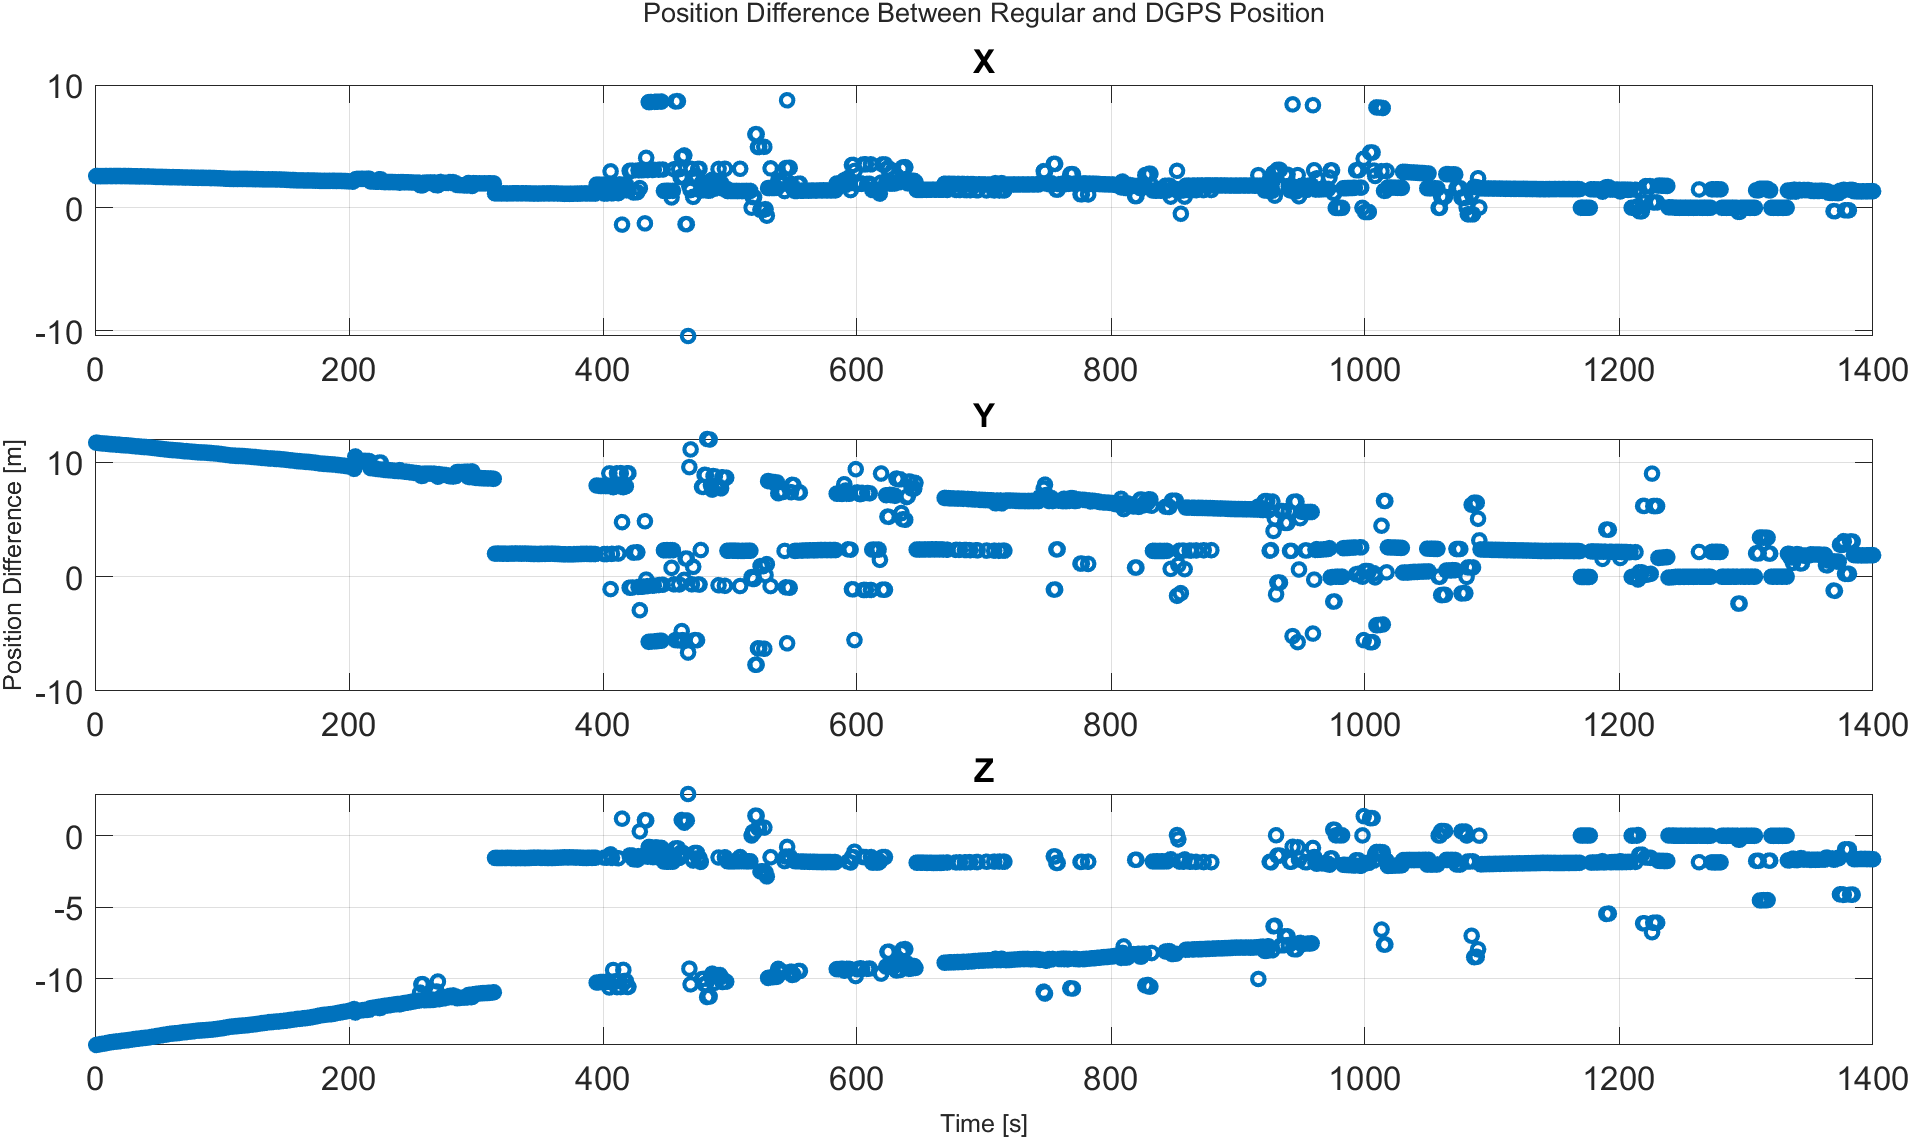
\includegraphics[width=0.85\textwidth]{p4_diff.png}
        \caption{WAAS Positioning Differences.}
      \end{figure}
      From \emph{Figures 18 and 19} it can be seen that the code DGPS solution closely 
      follows that of the original position solution. The difference in position never 
      goes above 15 meters of difference. This period of largest difference also occurs at 
      beginning of the run during a long period of no movement. In these static scenarios, 
      the code DGPS solution drifts since it has a greater noise component. Most of the 
      differences in positions while moving  between the two methods occurs during turns or 
      periods of terrain blockage. During these instants, the code DGPS solution sticks onto 
      the road as the original position solution drifts away. This can be seen better in 
      the right of \emph{Figure 18} where the DGPS position solution stays on the road during 
      tree blockage. It should also be noted that there are greater differences in the 
      y-direction than the x direction. This is likely due to the satellites being more 
      visible in that direction during the run, leading to less drift in that direction.
      % \begin{figure}[H]
      %   \centering
      %   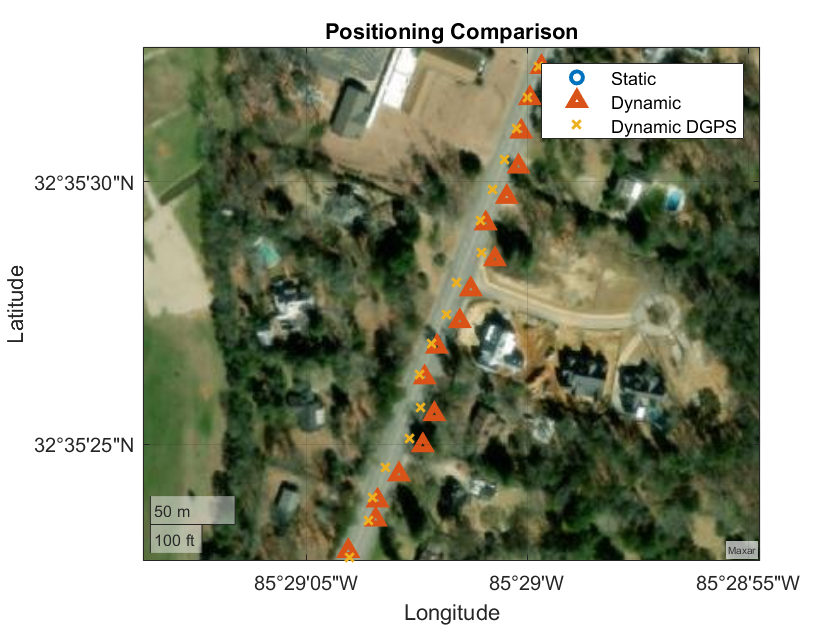
\includegraphics[width=0.85\textwidth]{p4_e.png}
      %   \caption{Zoomed in Comparison of Code DGPS and Original Position Solutions.}
      % \end{figure}

\end{enumerate}

\end{document}